% Options for packages loaded elsewhere
\PassOptionsToPackage{unicode}{hyperref}
\PassOptionsToPackage{hyphens}{url}
\documentclass[
  11pt,
]{article}
\usepackage{xcolor}
\usepackage[margin=2cm]{geometry}
\usepackage{amsmath,amssymb}
\setcounter{secnumdepth}{-\maxdimen} % remove section numbering
\usepackage{iftex}
\ifPDFTeX
  \usepackage[T1]{fontenc}
  \usepackage[utf8]{inputenc}
  \usepackage{textcomp} % provide euro and other symbols
\else % if luatex or xetex
  \usepackage{unicode-math} % this also loads fontspec
  \defaultfontfeatures{Scale=MatchLowercase}
  \defaultfontfeatures[\rmfamily]{Ligatures=TeX,Scale=1}
\fi
\usepackage{lmodern}
\ifPDFTeX\else
  % xetex/luatex font selection
\fi
% Use upquote if available, for straight quotes in verbatim environments
\IfFileExists{upquote.sty}{\usepackage{upquote}}{}
\IfFileExists{microtype.sty}{% use microtype if available
  \usepackage[]{microtype}
  \UseMicrotypeSet[protrusion]{basicmath} % disable protrusion for tt fonts
}{}
\makeatletter
\@ifundefined{KOMAClassName}{% if non-KOMA class
  \IfFileExists{parskip.sty}{%
    \usepackage{parskip}
  }{% else
    \setlength{\parindent}{0pt}
    \setlength{\parskip}{6pt plus 2pt minus 1pt}}
}{% if KOMA class
  \KOMAoptions{parskip=half}}
\makeatother
\usepackage{longtable,booktabs,array}
\usepackage{calc} % for calculating minipage widths
% Correct order of tables after \paragraph or \subparagraph
\usepackage{etoolbox}
\makeatletter
\patchcmd\longtable{\par}{\if@noskipsec\mbox{}\fi\par}{}{}
\makeatother
% Allow footnotes in longtable head/foot
\IfFileExists{footnotehyper.sty}{\usepackage{footnotehyper}}{\usepackage{footnote}}
\makesavenoteenv{longtable}
\setlength{\emergencystretch}{3em} % prevent overfull lines
\providecommand{\tightlist}{%
  \setlength{\itemsep}{0pt}\setlength{\parskip}{0pt}}
\usepackage{float}
\usepackage{caption}
\usepackage{tikz,pgfplots}
\usepackage{hyperref}
\pgfplotsset{compat=1.18}
\usepgfplotslibrary{groupplots}
\hypersetup{colorlinks=true,linkcolor=blue!50!black,urlcolor=blue!50!black}
\setlength{\emergencystretch}{3em}
\setlength{\parskip}{0.4em}
\pagestyle{plain}
\usepackage{bookmark}
\IfFileExists{xurl.sty}{\usepackage{xurl}}{} % add URL line breaks if available
\urlstyle{same}
\hypersetup{
  pdftitle={Encoder update location and nucleus-center detection: P20--P29},
  hidelinks,
  pdfcreator={LaTeX via pandoc}}

\title{Encoder update location and nucleus-center detection: P20--P29}
\author{}
\date{2026-11-15}

\begin{document}
\maketitle

{
\setcounter{tocdepth}{2}
\tableofcontents
}
P29 recovered 16/13 additional interior Dead nuclei in seeds 19/1 at the
original twelve-block update budget. Total matches increased by 283/165
and unmatched predictions decreased by 65/64. Both paired
image-bootstrap intervals are positive. Final Dead recall and precision
remain below the original absolute criteria. All four models completed
130 epochs and development evaluation. The last scheduler task reached
its time limit during preservation; a subsequent CPU job preserved and
verified both experimental seed-1 checkpoints and all result images.
Across this stage, updating encoder representations has produced more
consistent gains than the tested auxiliary supervision, parameter
averaging and weight constraint. The effect depends on which layers are
updated and which tissue images are considered.

\subsection{Data, matching and study
sequence}\label{data-matching-and-study-sequence}

Each round trains fresh controls and interventions from the same
pretrained UNI weights on 2,134 PanNuke fold-1 training images. The
epoch-130 checkpoint is evaluated on the same 522 development images
held out from that fold. Their 12,250 annotated nuclei define overall
recall. Precision uses every decoded center, including unmatched
predictions. One-to-one center matching uses a three-native-pixel
radius. The single output map predicts nucleus centers without class
labels; classes stratify the measured detections.

Interior Dead means the apoptotic/necrotic category with an annotated
outline clear of the image border: 145 nuclei on 11 images. The
small-object subset contains 32 objects with native area below 67
pixels. All comparisons retain seeds 19/1, the original split, decoding,
last-checkpoint rule and thresholds. Successive designs reuse this
development cohort. The tables describe within-round paired changes;
official instance-segmentation PQ and independent three-split evaluation
have their own protocol.

P30 was frozen before complete P29 seed-1 results, using P20--P28
evidence and P29 execution progress. It compares blocks 6--17 with
blocks 12--23 at equal trainable capacity. P29 remains on its original
allocation. The P30 acceptance and formal job receipt are documented
separately in \href{../P30_SUBMISSION.md}{P30\_SUBMISSION.md}.

\subsection{What the ten comparisons have
established}\label{what-the-ten-comparisons-have-established}

\begin{figure}[H]\centering
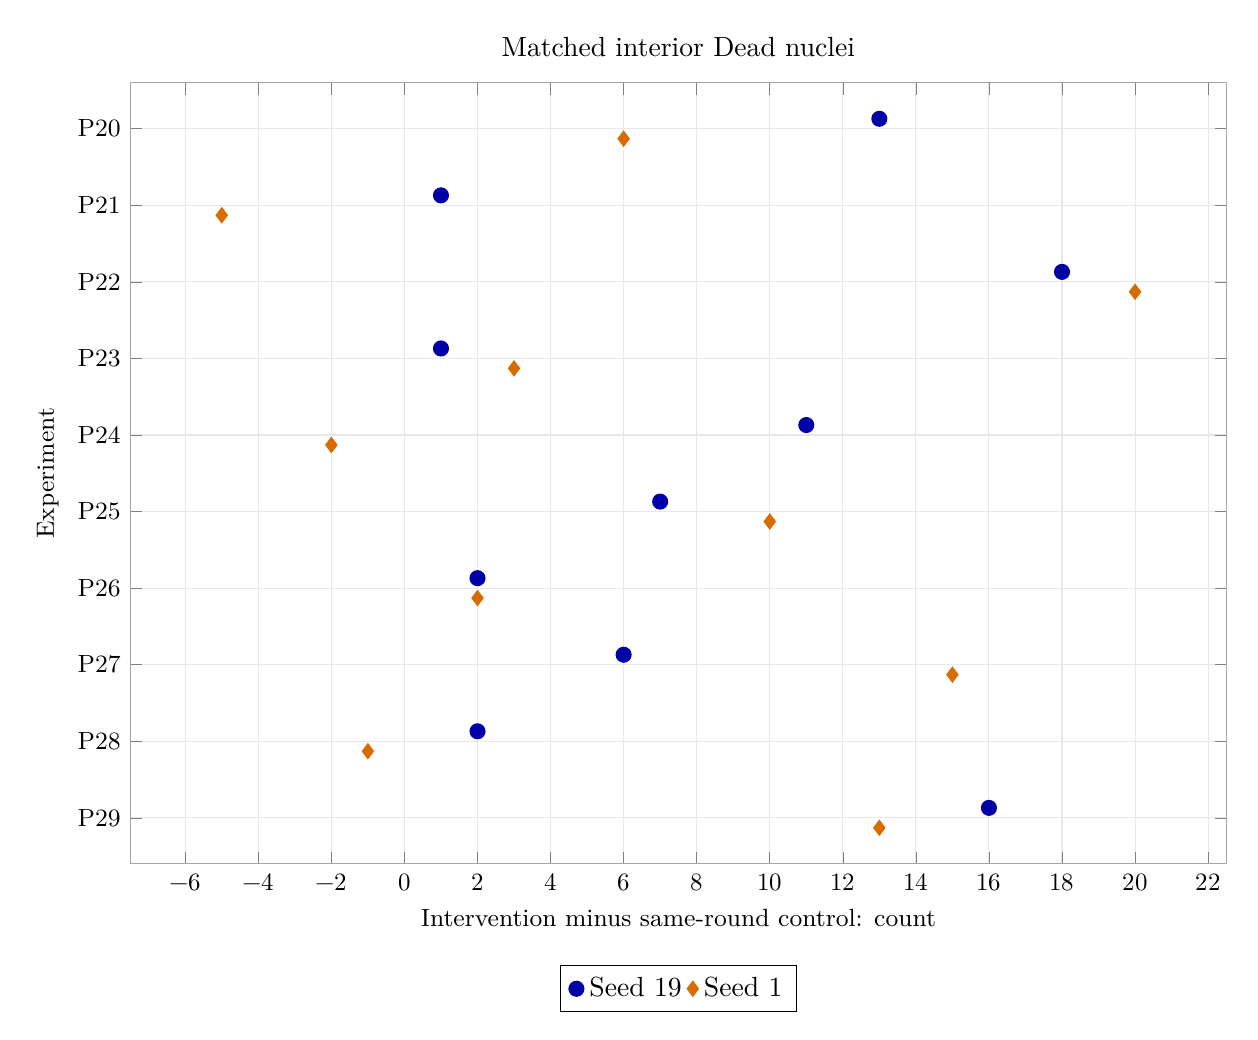
\begin{tikzpicture}
\begin{axis}[width=15.5cm,height=11.5cm,xlabel={Intervention minus same-round control: count},ylabel={Experiment},title={Matched interior Dead nuclei},ytick={0,1,2,3,4,5,6,7,8,9},yticklabels={P20,P21,P22,P23,P24,P25,P26,P27,P28,P29},ymin=-.6,ymax=9.6,y dir=reverse,grid=major,grid style={gray!18},legend style={at={(.5,-.13)},anchor=north,legend columns=2},axis line style={gray!70},tick label style={font=\small},label style={font=\small},title style={font=\normalsize}]
\addplot[only marks,mark=*,mark size=2.7pt,color=blue!65!black] coordinates {(13,-0.13) (1,0.87) (18,1.87) (1,2.87) (11,3.87) (7,4.87) (2,5.87) (6,6.87) (2,7.87) (16,8.87)};
\addlegendentry{Seed 19}
\addplot[only marks,mark=diamond*,mark size=2.7pt,color=orange!85!black] coordinates {(6,0.13) (-5,1.13) (20,2.13) (3,3.13) (-2,4.13) (10,5.13) (2,6.13) (15,7.13) (-1,8.13) (13,9.13)};
\addlegendentry{Seed 1}
\end{axis}
\end{tikzpicture}

\caption{Interior Dead changes, contemporaneous controls}
\end{figure}

\begin{figure}[H]\centering
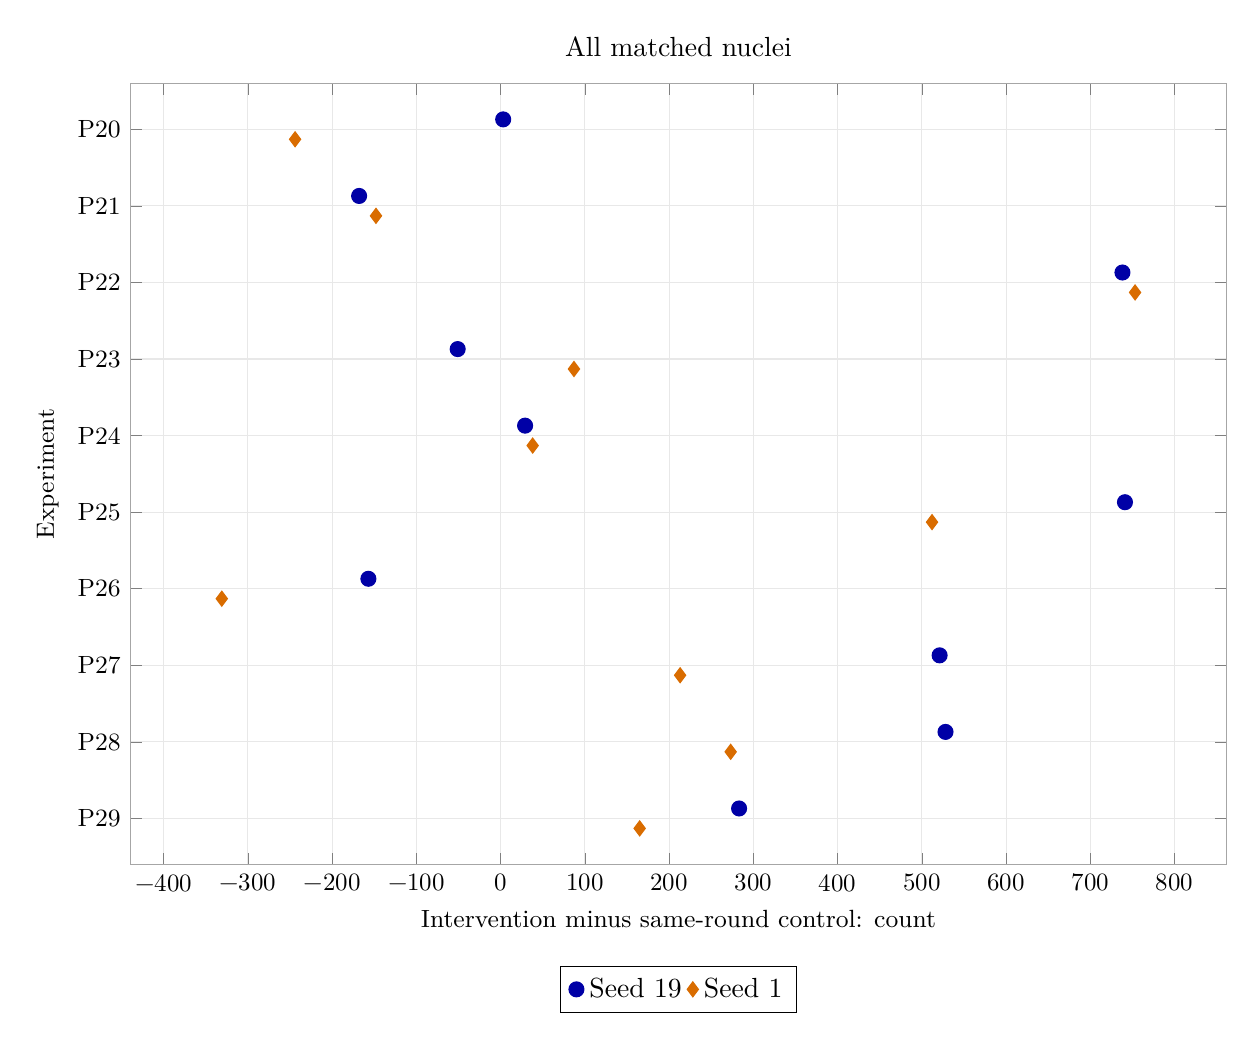
\begin{tikzpicture}
\begin{axis}[width=15.5cm,height=11.5cm,xlabel={Intervention minus same-round control: count},ylabel={Experiment},title={All matched nuclei},ytick={0,1,2,3,4,5,6,7,8,9},yticklabels={P20,P21,P22,P23,P24,P25,P26,P27,P28,P29},ymin=-.6,ymax=9.6,y dir=reverse,grid=major,grid style={gray!18},legend style={at={(.5,-.13)},anchor=north,legend columns=2},axis line style={gray!70},tick label style={font=\small},label style={font=\small},title style={font=\normalsize}]
\addplot[only marks,mark=*,mark size=2.7pt,color=blue!65!black] coordinates {(3,-0.13) (-168,0.87) (738,1.87) (-51,2.87) (29,3.87) (741,4.87) (-157,5.87) (521,6.87) (528,7.87) (283,8.87)};
\addlegendentry{Seed 19}
\addplot[only marks,mark=diamond*,mark size=2.7pt,color=orange!85!black] coordinates {(-244,0.13) (-148,1.13) (753,2.13) (87,3.13) (38,4.13) (512,5.13) (-331,6.13) (213,7.13) (273,8.13) (165,9.13)};
\addlegendentry{Seed 1}
\end{axis}
\end{tikzpicture}

\caption{Changes in all matched nuclei}
\end{figure}

\begin{figure}[H]\centering
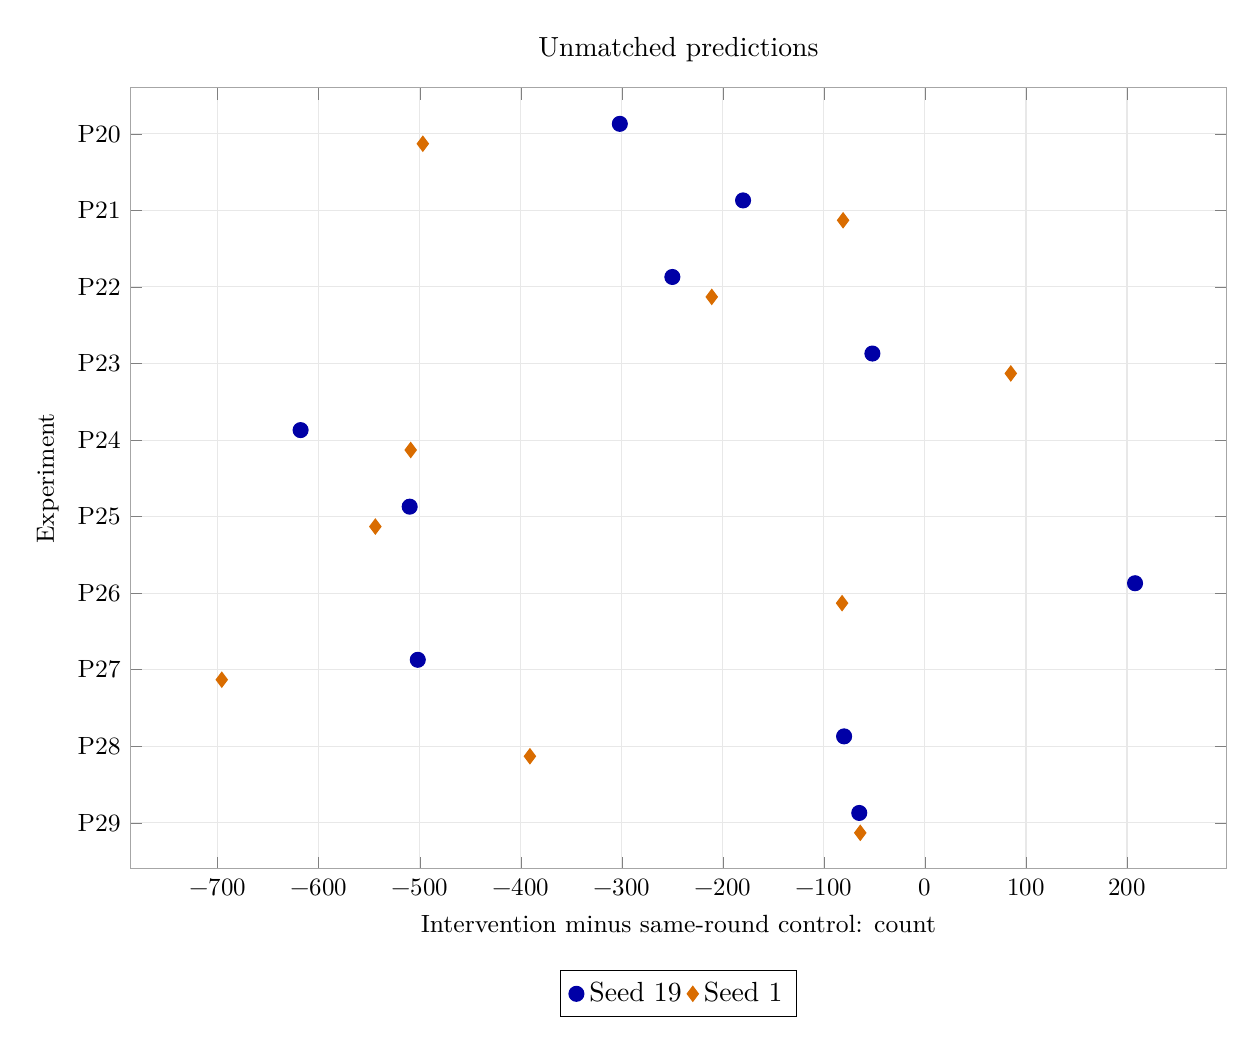
\begin{tikzpicture}
\begin{axis}[width=15.5cm,height=11.5cm,xlabel={Intervention minus same-round control: count},ylabel={Experiment},title={Unmatched predictions},ytick={0,1,2,3,4,5,6,7,8,9},yticklabels={P20,P21,P22,P23,P24,P25,P26,P27,P28,P29},ymin=-.6,ymax=9.6,y dir=reverse,grid=major,grid style={gray!18},legend style={at={(.5,-.13)},anchor=north,legend columns=2},axis line style={gray!70},tick label style={font=\small},label style={font=\small},title style={font=\normalsize}]
\addplot[only marks,mark=*,mark size=2.7pt,color=blue!65!black] coordinates {(-302,-0.13) (-180,0.87) (-250,1.87) (-52,2.87) (-618,3.87) (-510,4.87) (208,5.87) (-502,6.87) (-80,7.87) (-65,8.87)};
\addlegendentry{Seed 19}
\addplot[only marks,mark=diamond*,mark size=2.7pt,color=orange!85!black] coordinates {(-497,0.13) (-81,1.13) (-211,2.13) (85,3.13) (-509,4.13) (-544,5.13) (-82,6.13) (-696,7.13) (-391,8.13) (-64,9.13)};
\addlegendentry{Seed 1}
\end{axis}
\end{tikzpicture}

\caption{Changes in unmatched predictions}
\end{figure}

\begin{longtable}[]{@{}
  >{\raggedright\arraybackslash}p{(\linewidth - 6\tabcolsep) * \real{0.2000}}
  >{\raggedleft\arraybackslash}p{(\linewidth - 6\tabcolsep) * \real{0.2667}}
  >{\raggedleft\arraybackslash}p{(\linewidth - 6\tabcolsep) * \real{0.2667}}
  >{\raggedleft\arraybackslash}p{(\linewidth - 6\tabcolsep) * \real{0.2667}}@{}}
\toprule\noalign{}
\begin{minipage}[b]{\linewidth}\raggedright
Tested intervention
\end{minipage} & \begin{minipage}[b]{\linewidth}\raggedleft
Interior Dead matches, seeds 19 / 1
\end{minipage} & \begin{minipage}[b]{\linewidth}\raggedleft
All matches
\end{minipage} & \begin{minipage}[b]{\linewidth}\raggedleft
Unmatched predictions
\end{minipage} \\
\midrule\noalign{}
\endhead
\bottomrule\noalign{}
\endlastfoot
Input 512, P20 & +13 / +6 & +3 / −244 & −302 / −497 \\
Class-center supervision, P21 & +1 / −5 & −168 / −148 & −180 / −81 \\
All 24 encoder blocks, P22 & +18 / +20 & +738 / +753 & −250 / −211 \\
Parameter averaging, P23 & +1 / +3 & −51 / +87 & −52 / +85 \\
Higher late-block rate, P24 & +11 / −2 & +29 / +38 & −618 / −509 \\
All-block layerwise rates, P25 & +7 / +10 & +741 / +512 & −510 / −544 \\
Pretrained-weight constraint, P26 & +2 / +2 & −157 / −331 & +208 /
−82 \\
First 12 blocks, P27 & +6 / +15 & +521 / +213 & −502 / −696 \\
Alternating 12 blocks, P28 & +2 / −1 & +528 / +273 & −80 / −391 \\
First 6 + last 6 blocks, P29 & +16 / +13 & +283 / +165 & −65 / −64 \\
\end{longtable}

P20 found additional Dead nuclei through larger input images, but broad
coverage was inconsistent and training cost rose approximately 4.3-fold.
The spatial scale intervention therefore addresses a different tradeoff
from changing encoder update location. P21 reduced predictions and true
matches together. Its extra class-center targets did not improve
rare-object transfer under the tested fixed objective. P23's parameter
average changed few Dead matches and had mixed effects on total
coverage. P24 improved precision by removing many unmatched points, but
its rare-class gain reversed across seeds. These outcomes separate
prediction reduction from recovery of missing nuclei.

P22 produced the strongest consistent rare-class change: +18/+20
interior Dead matches, with +738/+753 total matches and fewer unmatched
predictions. Final Dead recall was 58.62\%/56.55\% and precision
72.84\%/73.36\%. Updating the full encoder improved the observed
detections while leaving the original absolute requirements unmet. P25
also improved broad coverage and precision, but smaller Dead gains
(+7/+10) came with tissue differences: lung gained 9/8 and colon lost
7/6. More total matches therefore do not imply consistent recovery of
the target class across tissues.

P26's pretrained-weight constraint reduced broad matching by 157/331
while adding two Dead matches per seed. Retaining parameters closer to
their initialization did not reproduce the full-depth response. P27,
with the same trainable parameter count as the late-block control,
gained 6/15 Dead matches and removed 502/696 unmatched predictions. Its
training recall dropped to 88.80\%/87.82\%. P28 restored training recall
to about 96.3\% by distributing updates across alternating layers, while
its rare-class change weakened to +2/−1. P29 seed 19 occupies another
point in this comparison: training recall is 95.47\% and rare-object
recovery rises by 16. These experiments establish update location as a
useful experimental variable. Training recall, trainable count and
distributed depth each leave part of the observed variation unexplained.
The representation mechanism remains a hypothesis.

\subsection{P29 seed 19: coverage, precision and
cost}\label{p29-seed-19-coverage-precision-and-cost}

\begin{longtable}[]{@{}
  >{\raggedright\arraybackslash}p{(\linewidth - 12\tabcolsep) * \real{0.1111}}
  >{\raggedleft\arraybackslash}p{(\linewidth - 12\tabcolsep) * \real{0.1481}}
  >{\raggedleft\arraybackslash}p{(\linewidth - 12\tabcolsep) * \real{0.1481}}
  >{\raggedleft\arraybackslash}p{(\linewidth - 12\tabcolsep) * \real{0.1481}}
  >{\raggedleft\arraybackslash}p{(\linewidth - 12\tabcolsep) * \real{0.1481}}
  >{\raggedleft\arraybackslash}p{(\linewidth - 12\tabcolsep) * \real{0.1481}}
  >{\raggedleft\arraybackslash}p{(\linewidth - 12\tabcolsep) * \real{0.1481}}@{}}
\toprule\noalign{}
\begin{minipage}[b]{\linewidth}\raggedright
Allocation
\end{minipage} & \begin{minipage}[b]{\linewidth}\raggedleft
Interior Dead
\end{minipage} & \begin{minipage}[b]{\linewidth}\raggedleft
Small Dead
\end{minipage} & \begin{minipage}[b]{\linewidth}\raggedleft
All matched
\end{minipage} & \begin{minipage}[b]{\linewidth}\raggedleft
Recall
\end{minipage} & \begin{minipage}[b]{\linewidth}\raggedleft
Precision
\end{minipage} & \begin{minipage}[b]{\linewidth}\raggedleft
Unmatched
\end{minipage} \\
\midrule\noalign{}
\endhead
\bottomrule\noalign{}
\endlastfoot
Last 12 blocks & 65/145 & 7/32 & 7,257/12,250 & 59.24\% & 69.73\% &
3,150 \\
First 6 + last 6 & 81/145 & 11/32 & 7,540/12,250 & 61.55\% & 70.96\% &
3,085 \\
\end{longtable}

The intervention emitted 218 more points while finding 283 more nuclei.
This combination reflects more useful predictions rather than a simple
increase in output count. Interior Dead recall rose 11.0345 percentage
points, with the unchanged 1,000-draw tissue-stratified bootstrap
interval {[}+3.0457,+27.9570{]} points. Overall recall rose 2.3102
points and precision 1.2328 points. The original seed-level conjunction
fails the absolute Dead recall (.60) and precision (.75) clauses; all
other seed-19 clauses pass. The seed-1 comparison independently improves
Dead recall by 8.9655 percentage points and also fails the same two
absolute clauses.

Training recall changed 97.51\%→95.47\% and training Dead coverage
630/656→607/656. Pure training took 4.0130 versus 4.8652 hours, a
21.24\% increase. Peak allocated GPU memory was 4.05 versus 4.84 GiB.
Completed seed-19 scheduler elapsed time was 4:13:24 plus 5:00:21,
including startup, evaluation and preservation. These measurements price
the twelve-block intervention without substituting training fit for
development performance.

\begin{figure}[H]\centering
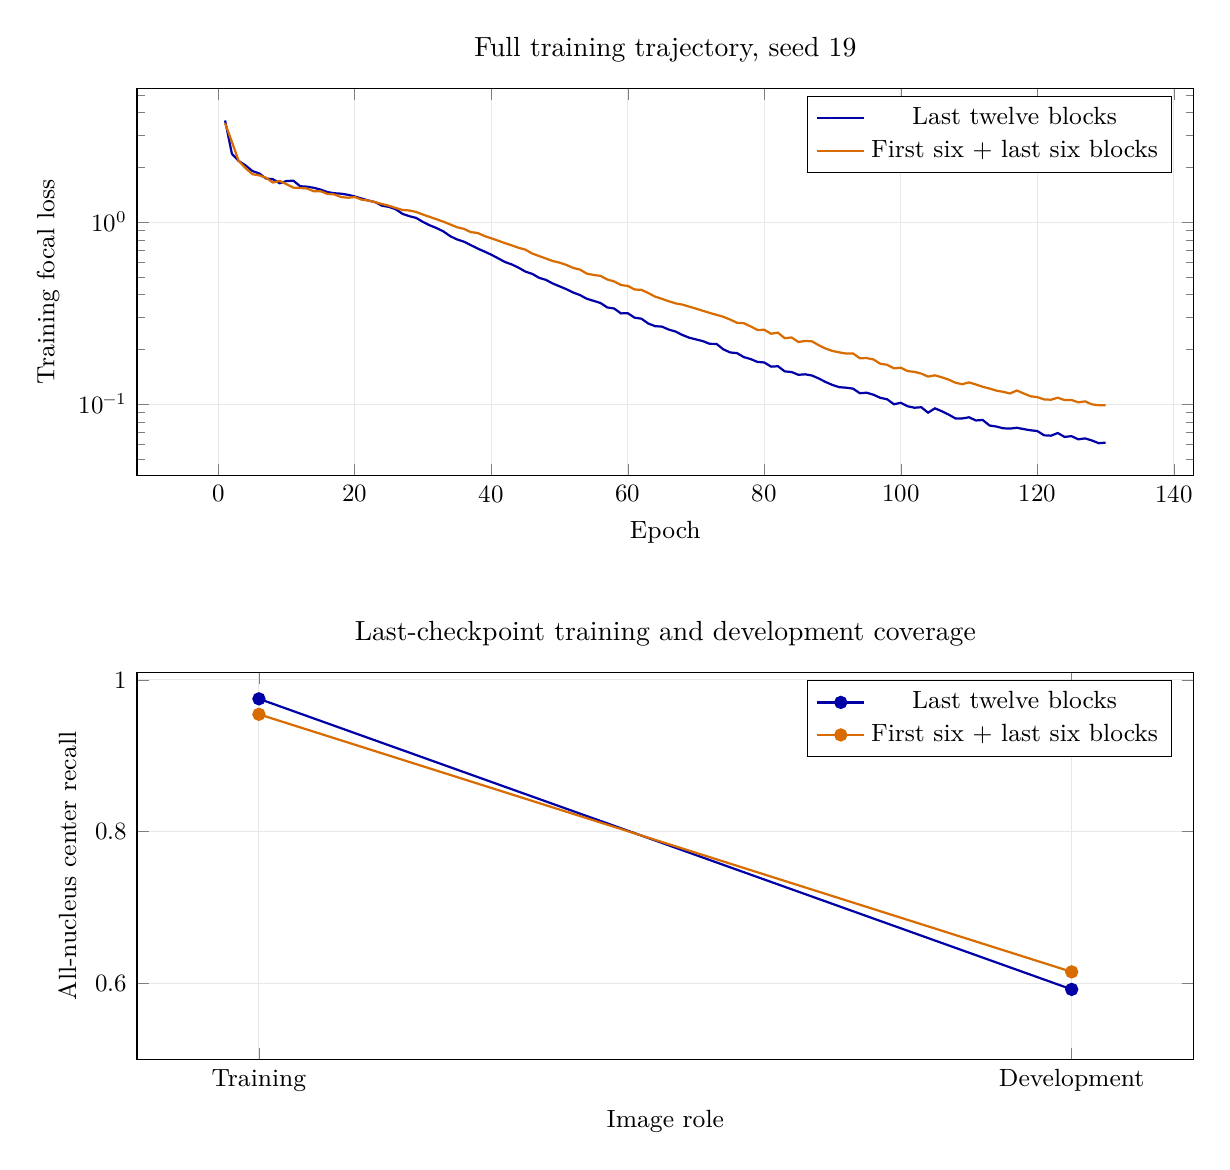
\begin{tikzpicture}
\begin{groupplot}[group style={group size=1 by 2,vertical sep=2.5cm},width=15cm,height=6.5cm,grid=major,grid style={gray!18},legend style={font=\small},tick label style={font=\small},label style={font=\small},title style={font=\normalsize}]
\nextgroupplot[xlabel={Epoch},ylabel={Training focal loss},ymode=log,title={Full training trajectory, seed 19}]
\addplot[thick,color=blue!65!black] coordinates {(1,3.62386978209) (2,2.37552843165) (3,2.1699790582) (4,2.05083011871) (5,1.91124379869) (6,1.85306071716) (7,1.73830157976) (8,1.72317317723) (9,1.63716908066) (10,1.68299786846) (11,1.69219968882) (12,1.57655350178) (13,1.56793110214) (14,1.54554083125) (15,1.51068508564) (16,1.46400284926) (17,1.44252403023) (18,1.43446976444) (19,1.41490890473) (20,1.38527809719) (21,1.34936290868) (22,1.31520210644) (23,1.28915614926) (24,1.23129468712) (25,1.21430525547) (26,1.17777008382) (27,1.11140446291) (28,1.07907247314) (29,1.05578593797) (30,1.00256185944) (31,0.961115168291) (32,0.927977368473) (33,0.889346529835) (34,0.837489534103) (35,0.803761817047) (36,0.781447936886) (37,0.748062575356) (38,0.716612512178) (39,0.690093925696) (40,0.662901303416) (41,0.633349982007) (42,0.604437001957) (43,0.586148878439) (44,0.56240585762) (45,0.535049840808) (46,0.52007716346) (47,0.494900800501) (48,0.482175430491) (49,0.460473351715) (50,0.444158400534) (51,0.428483899194) (52,0.410752979311) (53,0.397682718374) (54,0.379469061984) (55,0.369665312337) (56,0.3597513164) (57,0.339892074871) (58,0.3355475312) (59,0.315381314616) (60,0.316084984617) (61,0.29880171501) (62,0.294916734044) (63,0.277473928217) (64,0.268344895773) (65,0.266779590272) (66,0.256976687361) (67,0.250711295104) (68,0.239990992582) (69,0.231839629632) (70,0.22687595172) (71,0.222037940652) (72,0.214563905512) (73,0.214325386403) (74,0.200130272068) (75,0.192422631313) (76,0.190850315003) (77,0.181378530923) (78,0.176991748792) (79,0.170684004576) (80,0.169478886474) (81,0.160782273263) (82,0.161583742678) (83,0.151403813556) (84,0.150206022232) (85,0.145022003989) (86,0.145890951062) (87,0.143605590676) (88,0.138312381576) (89,0.132313917474) (90,0.127416898005) (91,0.123964854301) (92,0.123164128256) (93,0.121683641281) (94,0.114873931265) (95,0.115586895261) (96,0.11267241873) (97,0.108353732171) (98,0.106374115275) (99,0.0999097410195) (100,0.101763770482) (101,0.0973861433292) (102,0.0956012586589) (103,0.0961770233598) (104,0.0898133710938) (105,0.0948688865752) (106,0.0914647224007) (107,0.0876876159738) (108,0.0835042551837) (109,0.0834624404777) (110,0.0847086207095) (111,0.081374704054) (112,0.0818419124579) (113,0.0763423845631) (114,0.0753366971919) (115,0.0736962775521) (116,0.073428697569) (117,0.0741943524436) (118,0.072946563604) (119,0.0718636737304) (120,0.0711843375659) (121,0.0674173853084) (122,0.0671176563974) (123,0.0693980144741) (124,0.0660580317782) (125,0.0667165935397) (126,0.0640829772725) (127,0.0648491781496) (128,0.0631586541985) (129,0.0610245662421) (130,0.0614443497449)};
\addlegendentry{Last twelve blocks}
\addplot[thick,color=orange!85!black] coordinates {(1,3.50105492356) (2,2.76289148384) (3,2.17038305907) (4,1.98312889879) (5,1.83590344865) (6,1.80892446338) (7,1.75439191267) (8,1.65186924516) (9,1.68502842514) (10,1.6174624693) (11,1.54911897966) (12,1.54232221831) (13,1.53134093183) (14,1.4787512504) (15,1.47922120177) (16,1.42957731283) (17,1.42129815264) (18,1.37443559306) (19,1.36327421378) (20,1.37542054736) (21,1.33016328574) (22,1.31518258203) (23,1.28756736924) (24,1.25844964483) (25,1.23172492314) (26,1.19774090467) (27,1.16697317507) (28,1.15981375325) (29,1.1382047245) (30,1.10121632304) (31,1.06901810135) (32,1.03754835332) (33,1.00610931113) (34,0.971616917315) (35,0.937913104096) (36,0.919036173231) (37,0.881783900411) (38,0.87277482538) (39,0.839935905931) (40,0.815554868329) (41,0.792132447564) (42,0.767330217063) (43,0.746182883663) (44,0.723307935652) (45,0.706632291631) (46,0.672832300026) (47,0.65200705931) (48,0.63159530658) (49,0.61198255419) (50,0.599476133104) (51,0.582289886012) (52,0.560812200321) (53,0.548834211698) (54,0.521759605494) (55,0.512614208503) (56,0.507201689686) (57,0.484308340912) (58,0.472578119371) (59,0.451809032474) (60,0.446398185728) (61,0.426876144423) (62,0.424710518125) (63,0.408310935512) (64,0.390026470253) (65,0.379042657953) (66,0.36809506068) (67,0.358036929659) (68,0.352404804322) (69,0.343642305939) (70,0.334936154565) (71,0.325884575944) (72,0.317293170609) (73,0.309748381034) (74,0.302111506041) (75,0.291821877321) (76,0.279997927729) (77,0.278499311239) (78,0.26754597844) (79,0.255842017163) (80,0.256262032252) (81,0.243800983989) (82,0.247128760941) (83,0.230332737019) (84,0.232489445869) (85,0.219672735791) (86,0.222537847046) (87,0.221399081085) (88,0.210550299569) (89,0.202055267706) (90,0.196092654535) (91,0.192539622031) (92,0.189735345935) (93,0.189959515611) (94,0.178786053381) (95,0.179221209236) (96,0.176041919675) (97,0.166773603559) (98,0.164553097721) (99,0.157313765623) (100,0.158646976891) (101,0.151932625451) (102,0.150512845719) (103,0.147210237615) (104,0.141779869506) (105,0.144020077068) (106,0.140556078439) (107,0.136488059869) (108,0.131228308264) (109,0.12870185654) (110,0.13169746431) (111,0.128227441007) (112,0.124542114723) (113,0.12187337539) (114,0.118651823402) (115,0.116943936811) (116,0.114445477206) (117,0.118868027916) (118,0.114558337975) (119,0.110518558363) (120,0.109255300938) (121,0.10619787934) (122,0.105784444191) (123,0.108507285318) (124,0.105264322801) (125,0.105468319092) (126,0.102285939834) (127,0.10359711623) (128,0.0997327014371) (129,0.0986843192636) (130,0.0987533847518)};
\addlegendentry{First six + last six blocks}
\nextgroupplot[xlabel={Image role},ylabel={All-nucleus center recall},title={Last-checkpoint training and development coverage},xtick={0,1},xticklabels={Training,Development},xmin=-.15,xmax=1.15,ymin=.5,ymax=1.01]
\addplot[thick,mark=*,color=blue!65!black] coordinates {(0,0.975082404646) (1,0.592408163265)};
\addlegendentry{Last twelve blocks}
\addplot[thick,mark=*,color=orange!85!black] coordinates {(0,0.954697064825) (1,0.615510204082)};
\addlegendentry{First six + last six blocks}
\end{groupplot}
\end{tikzpicture}

\caption{Full trajectory and coverage at epoch 130}
\end{figure}

\subsection{Tissue distribution and
sensitivity}\label{tissue-distribution-and-sensitivity}

\begin{figure}[H]\centering
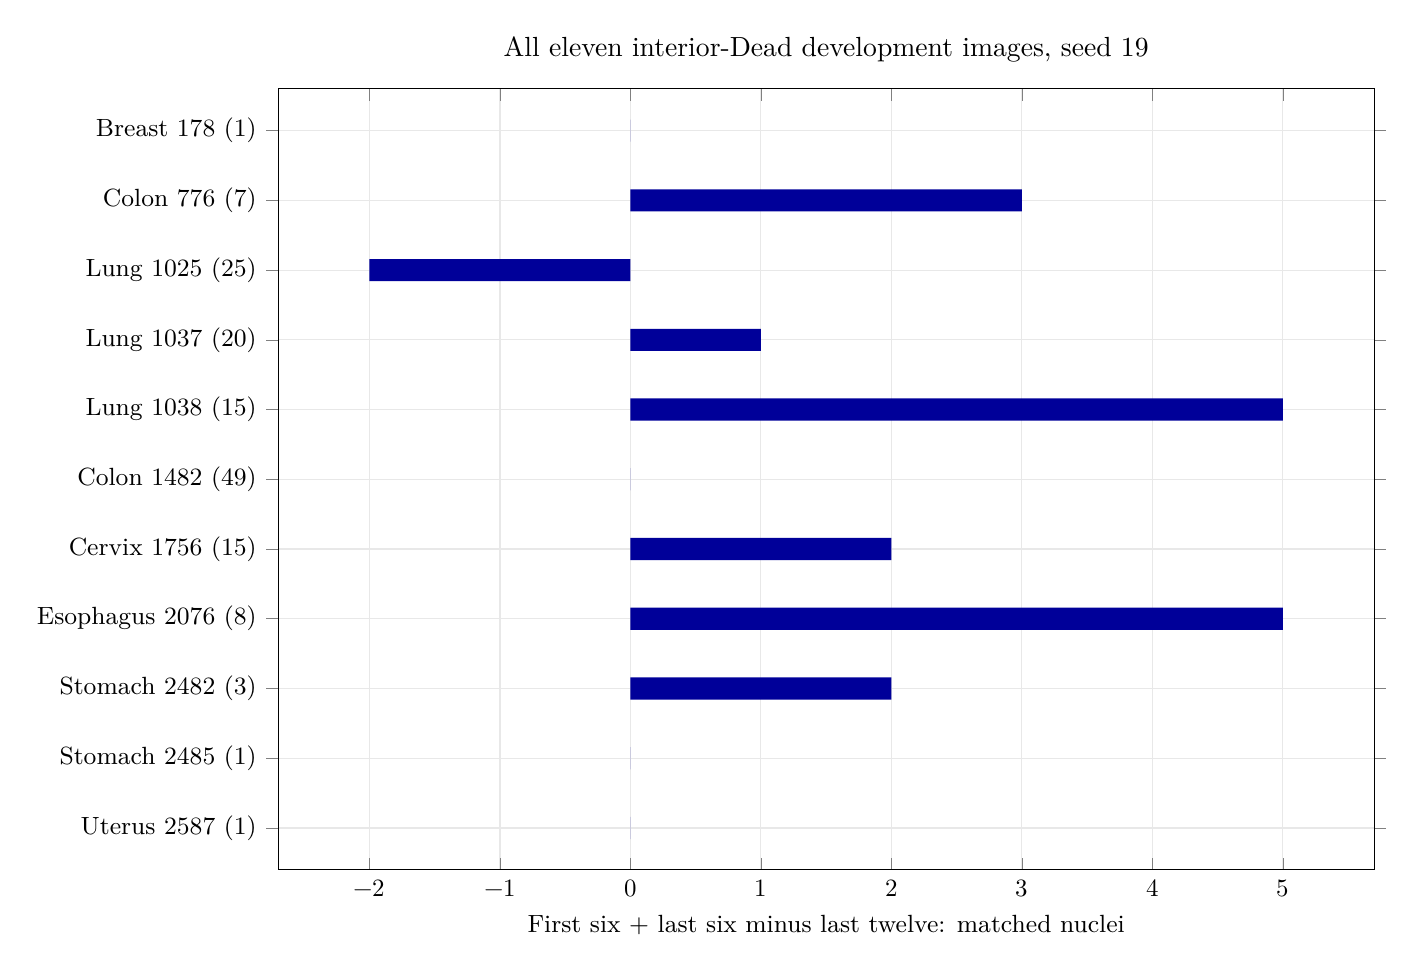
\begin{tikzpicture}
\begin{axis}[xbar,width=15.5cm,height=11.5cm,xlabel={First six + last six minus last twelve: matched nuclei},title={All eleven interior-Dead development images, seed 19},ytick={0,1,2,3,4,5,6,7,8,9,10},yticklabels={{Breast 178 (1)},{Colon 776 (7)},{Lung 1025 (25)},{Lung 1037 (20)},{Lung 1038 (15)},{Colon 1482 (49)},{Cervix 1756 (15)},{Esophagus 2076 (8)},{Stomach 2482 (3)},{Stomach 2485 (1)},{Uterus 2587 (1)}},ymin=-.6,ymax=10.6,y dir=reverse,bar width=8pt,grid=major,grid style={gray!18},tick label style={font=\small},label style={font=\small},title style={font=\normalsize}]
\addplot[fill=blue!60!black,draw=none] coordinates {(0,0) (3,1) (-2,2) (1,3) (5,4) (0,5) (2,6) (5,7) (2,8) (0,9) (0,10)};
\end{axis}
\end{tikzpicture}

\caption{All eleven images with interior Dead annotations}
\end{figure}

Six images gained matches, one lost matches and four were unchanged.
Lung changed +4, colon +3, cervix +2, esophagus +5 and stomach +2;
breast and uterus were unchanged. Lung image 1038 and esophagus image
2076 each gained five, together accounting for 10/16 net gains. Lung
image 1025 lost two despite aggregate lung improvement. Colon image 1482
contains 49/145 target objects and stays at 13 matches in both arms,
leaving 36 unmatched target objects in that image.

Removing one Dead-positive image at a time, solely as a sensitivity
calculation, leaves gains between 8.03\% and 16.67\%. Every such gain
remains positive. The observed seed-19 sign consequently survives
omission of any one contributing image; the full original decision still
includes all eleven images. A tissue with one positive image offers
limited evidence for between-image consistency within that tissue.

\subsection{Fixed images: which annotated nuclei
changed}\label{fixed-images-which-annotated-nuclei-changed}

The pre-fixed eight evaluation examples contain 53 interior Dead nuclei.
Seed 19 retained 30, gained 6, lost 4 and missed 13 in both arms. Their
net change is +2, versus +16 across all 522 evaluation images. Object
indices and row,column coordinates are retained in
\href{../fixed_objects.csv}{fixed\_objects.csv}. Cyan crosses show all
predictions; shared white, green, orange and pink rings respectively
identify retained, gained, lost and jointly missed target objects.

\noindent

\begin{minipage}{\linewidth}\centering
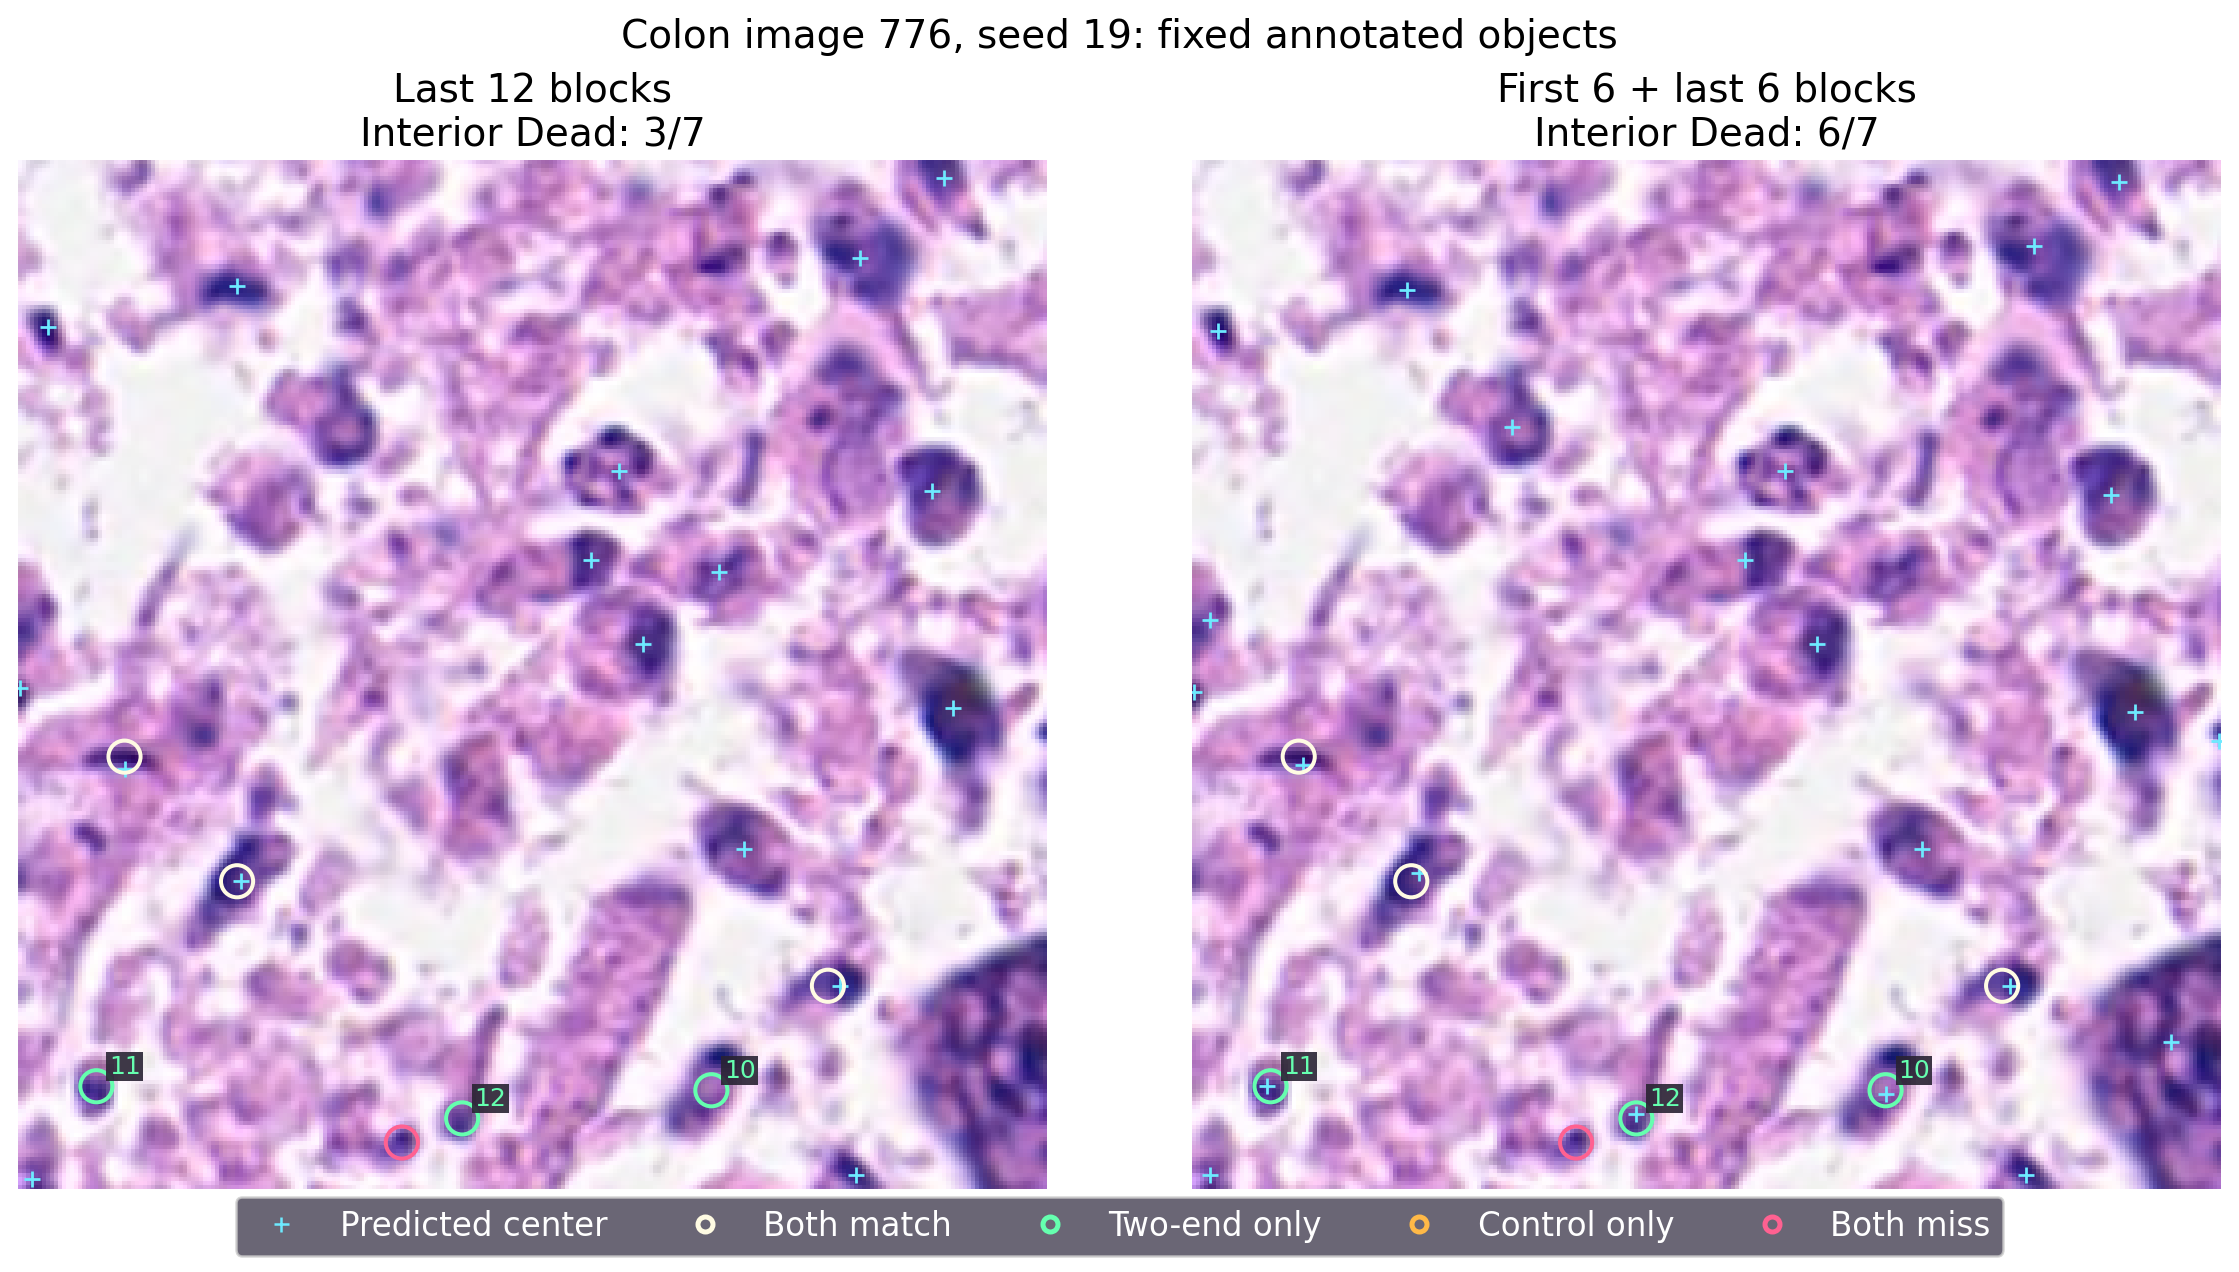
\includegraphics[width=\linewidth,height=0.40\textheight,keepaspectratio]{../figures/p29_image_776_seed_19.png}
\captionof{figure}{Colon image 776, fixed seed-19 comparison}
\raggedright

Colon image 776 changes from 3/7 to 6/7 target matches. Three gained objects lie in the lower tissue strip: object 10 at (231,172), object 11 at (230,19), and object 12 at (238,110). Their nearest decoded-point distances change 41.23→1.00, 28.02→1.00 and 80.66→1.00 pixels. The right panel places predictions close to all three annotations; the control has no decoded point in their immediate neighborhoods. Their visible size and pale appearance vary, and object 12 has area 104 pixels. This is recovery beyond the smallest predefined size bin.

\end{minipage}

\noindent

\begin{minipage}{\linewidth}\centering
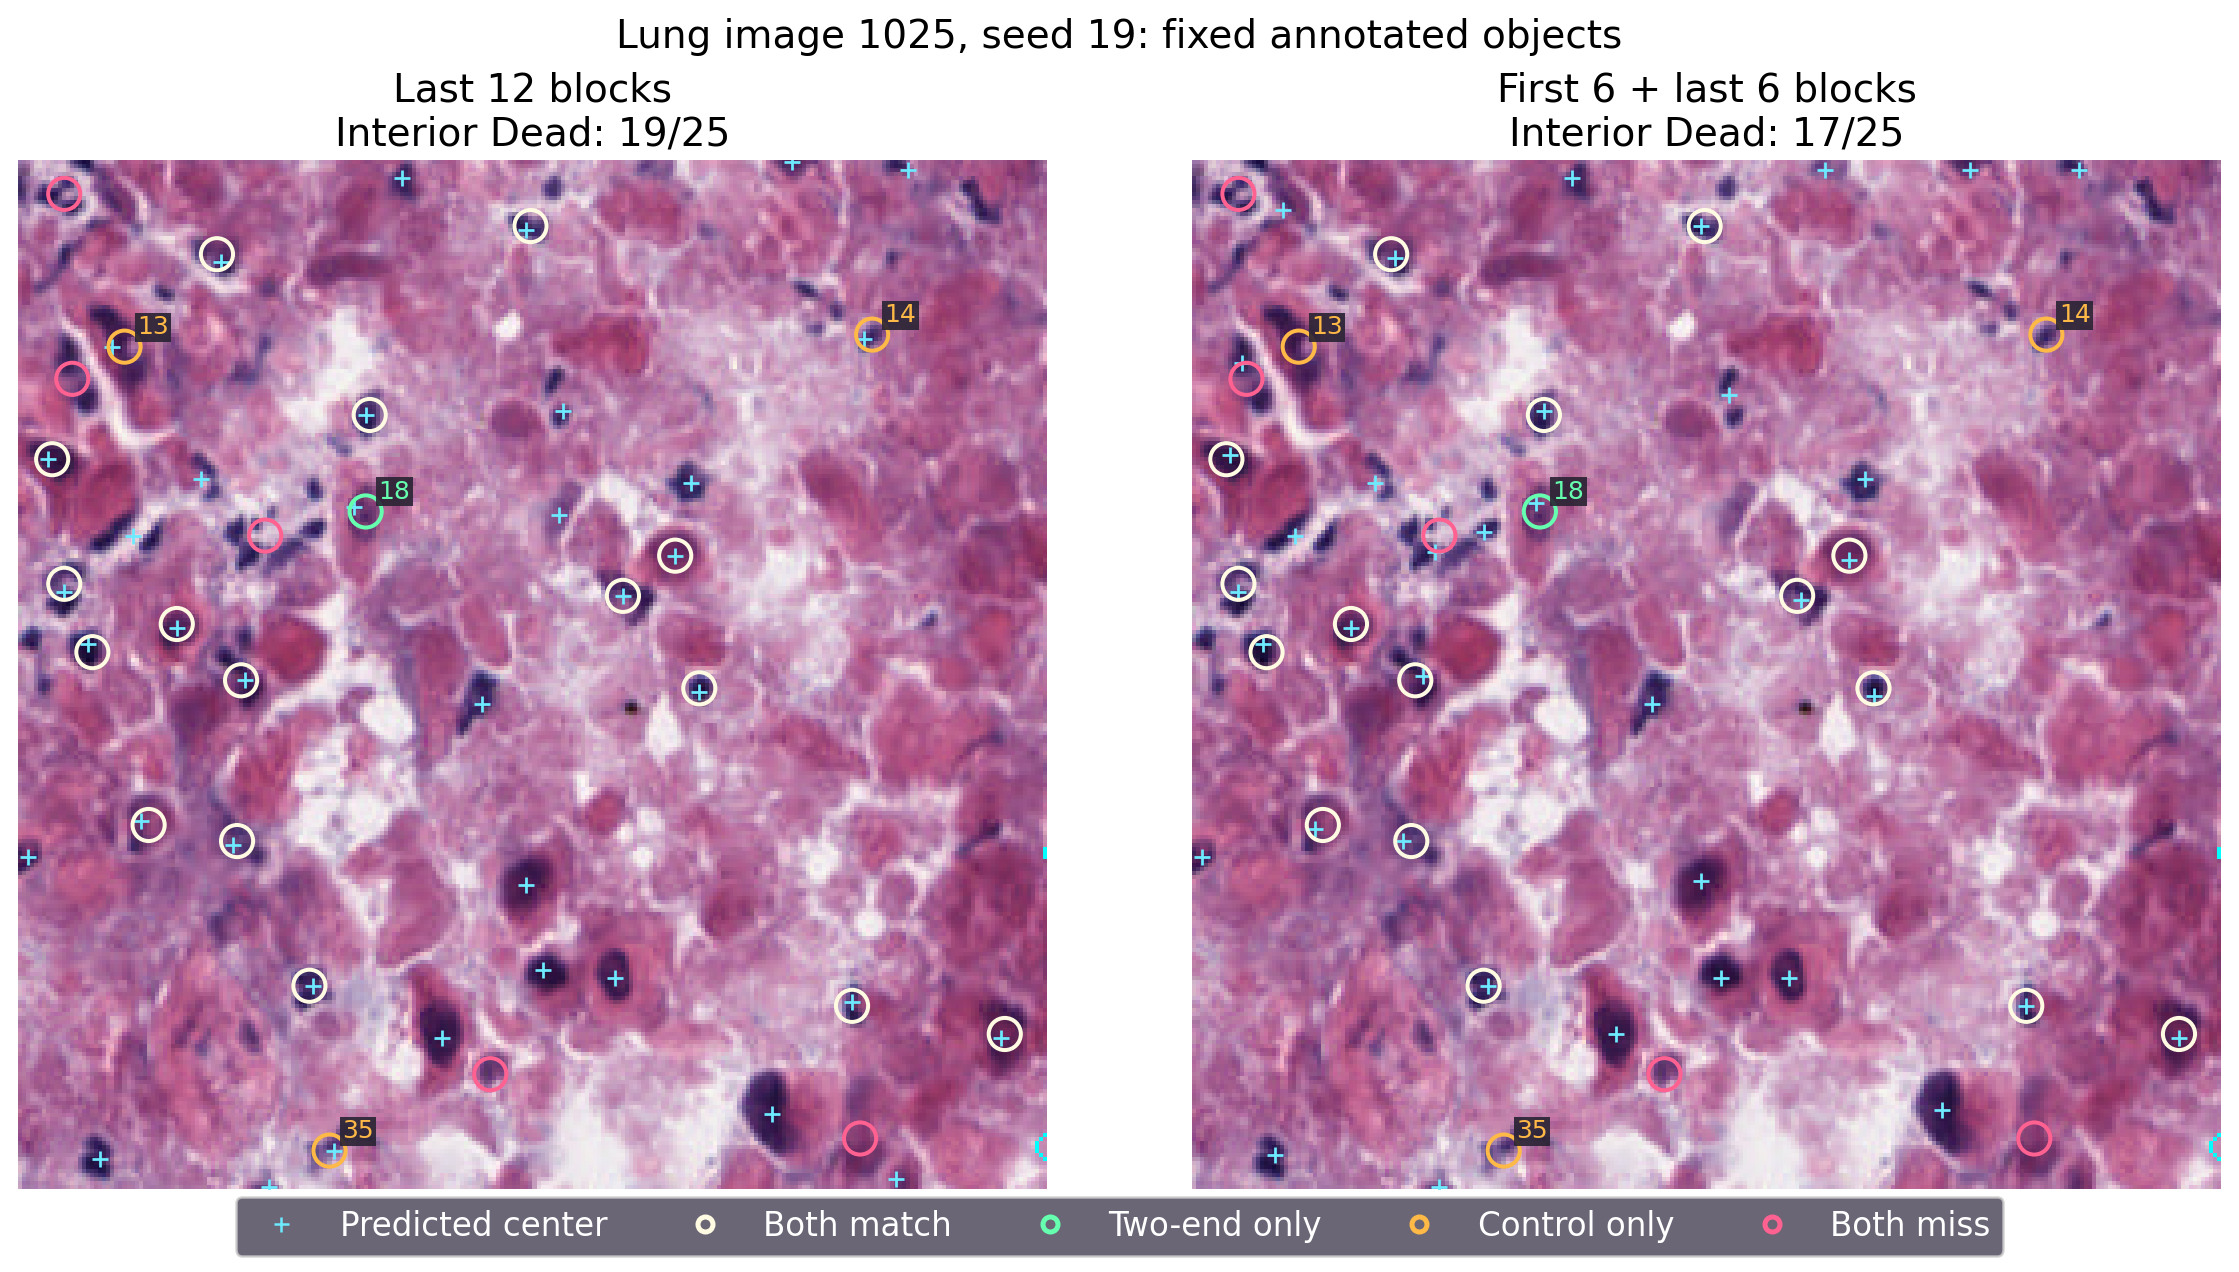
\includegraphics[width=\linewidth,height=0.40\textheight,keepaspectratio]{../figures/p29_image_1025_seed_19.png}
\captionof{figure}{Lung image 1025: gains alongside lost detections}
\raggedright

Lung image 1025 changes from 19/25 to 17/25. Object 18 at (87,86) gains a match as its nearest point moves from 3.16 to 2.24 pixels, crossing the fixed three-pixel matching boundary. Objects 13 at (46,26), 14 at (43,212), and 35 at (246,77) lose matches, with nearest distances 3.00→14.56, 2.24→41.77 and 1.00→18.36. Object 14 has area 31 pixels and is visibly small. The intervention removes useful outputs around these annotations while recovering another object. The full tissue aggregate cannot reveal this exchange.

\end{minipage}

\noindent

\begin{minipage}{\linewidth}\centering
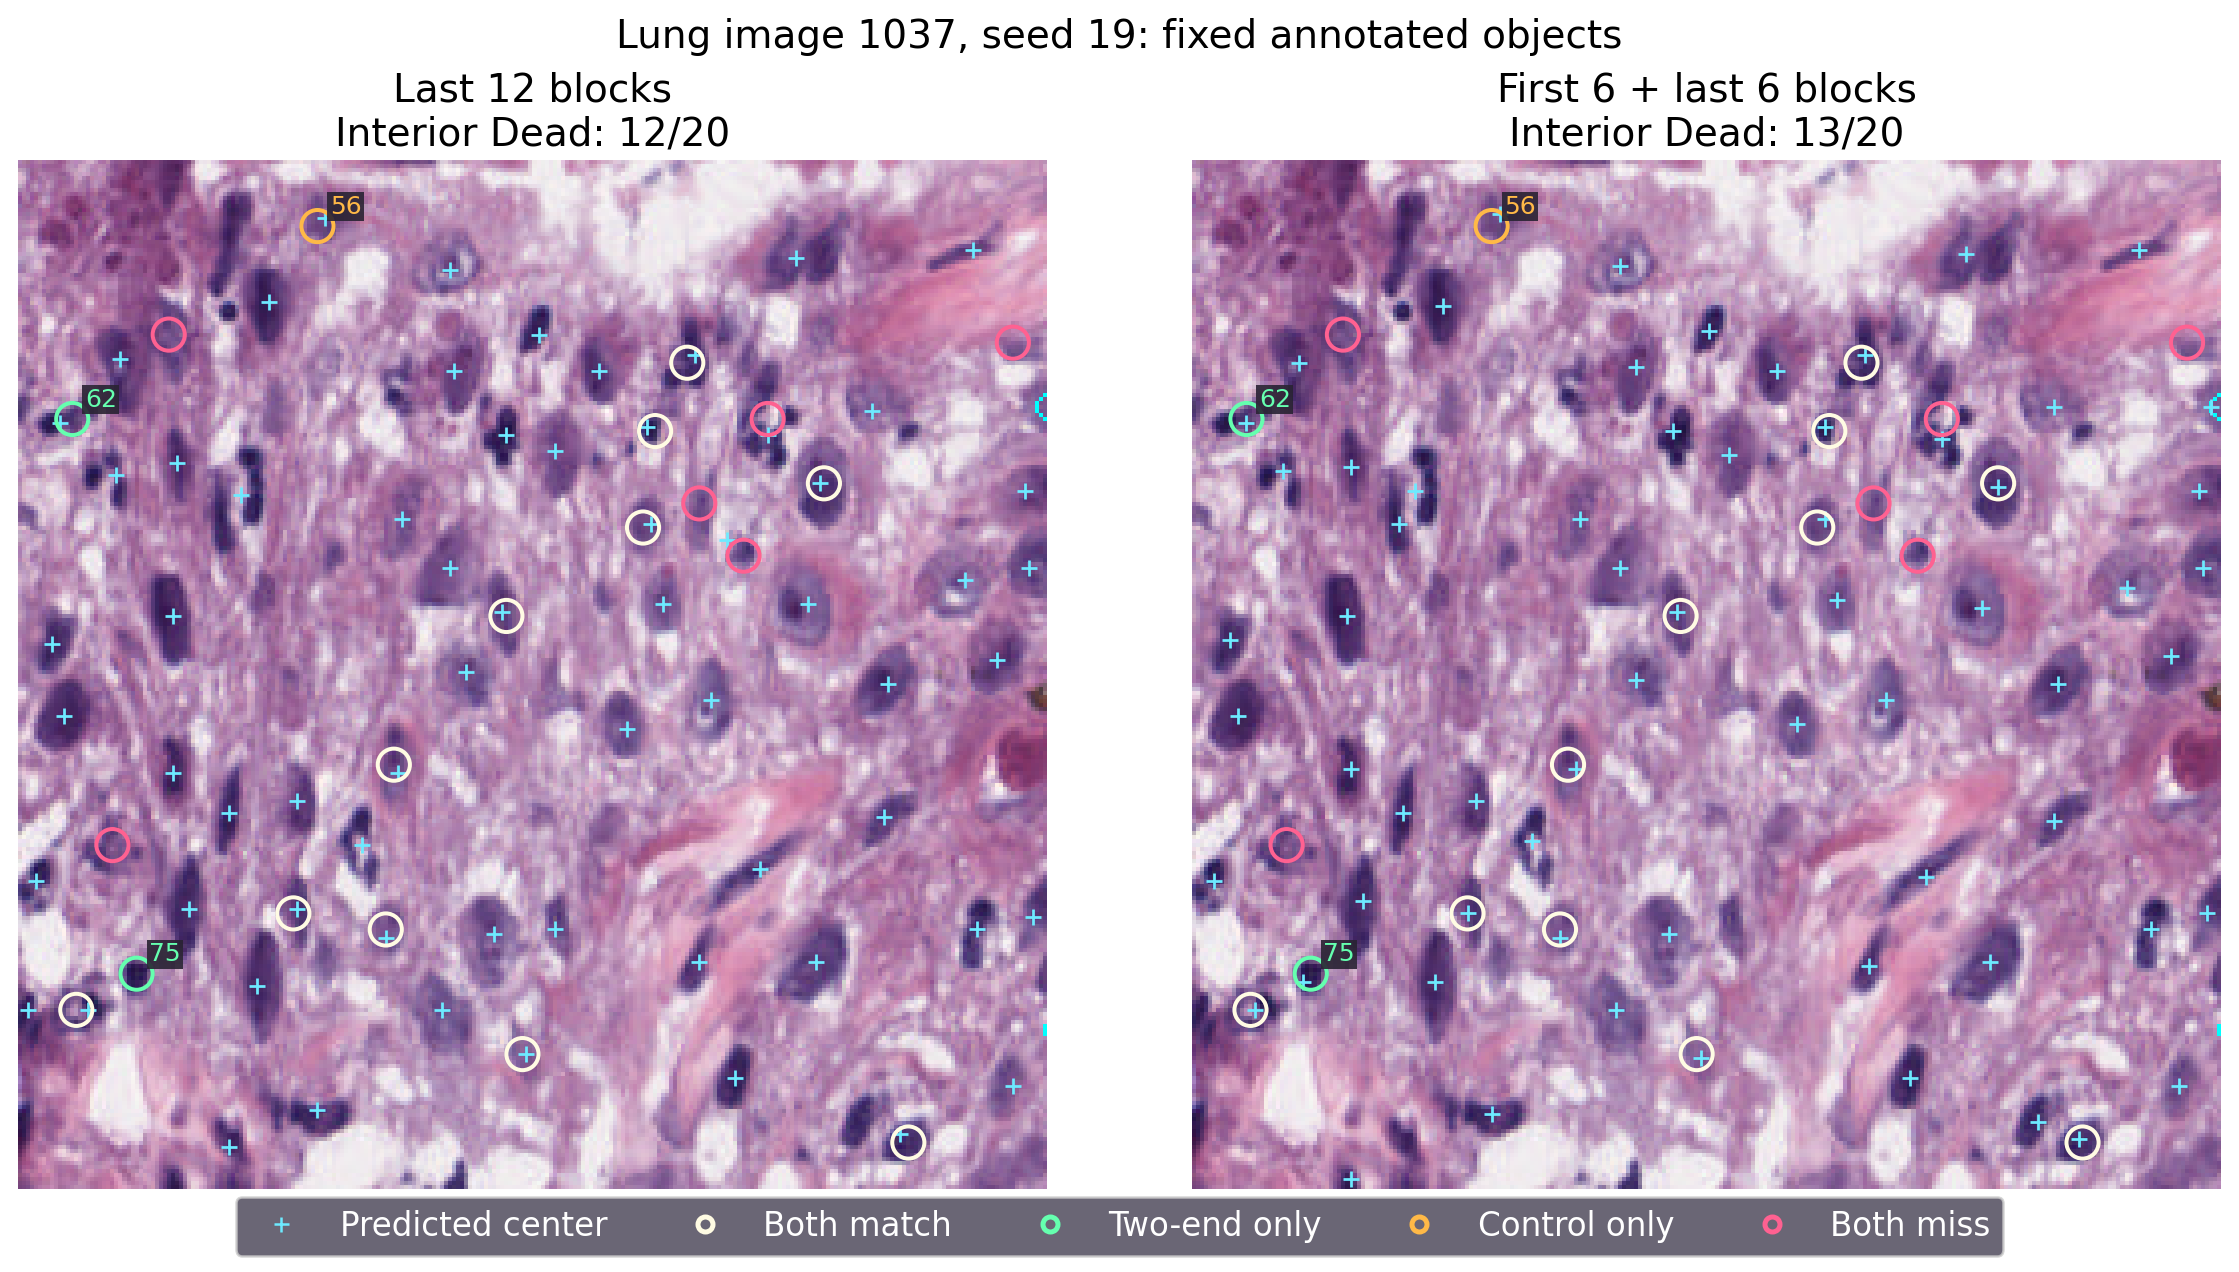
\includegraphics[width=\linewidth,height=0.40\textheight,keepaspectratio]{../figures/p29_image_1037_seed_19.png}
\captionof{figure}{Lung image 1037: a larger gain and a boundary displacement}
\raggedright

Lung image 1037 changes from 12/20 to 13/20. Object 62 at (64,13) gains a match as nearest distance falls 3.16→1.00; object 75 at (202,29), area 44 pixels, changes 15.00→2.83. Object 56 at (16,74) loses its match after a nearby point shifts from 2.83 to 3.61 pixels. The latter event is a displacement across the matching radius; the former small-object gain places a prediction in a previously uncovered neighborhood.

\end{minipage}

Coordinates establish appearance, disappearance and displacement of
decoded points. Image intensity and tissue context make these events
visible. Attribution to center-score strength, peak suppression or
hidden encoder features requires probability maps or intermediate
measurements; this collection stores original images, annotated centers,
decoded points and one-to-one assignments.

\subsection{Seed 1 and consistency across
seeds}\label{seed-1-and-consistency-across-seeds}

\begin{longtable}[]{@{}
  >{\raggedright\arraybackslash}p{(\linewidth - 12\tabcolsep) * \real{0.1111}}
  >{\raggedleft\arraybackslash}p{(\linewidth - 12\tabcolsep) * \real{0.1481}}
  >{\raggedleft\arraybackslash}p{(\linewidth - 12\tabcolsep) * \real{0.1481}}
  >{\raggedleft\arraybackslash}p{(\linewidth - 12\tabcolsep) * \real{0.1481}}
  >{\raggedleft\arraybackslash}p{(\linewidth - 12\tabcolsep) * \real{0.1481}}
  >{\raggedleft\arraybackslash}p{(\linewidth - 12\tabcolsep) * \real{0.1481}}
  >{\raggedleft\arraybackslash}p{(\linewidth - 12\tabcolsep) * \real{0.1481}}@{}}
\toprule\noalign{}
\begin{minipage}[b]{\linewidth}\raggedright
Seed / allocation
\end{minipage} & \begin{minipage}[b]{\linewidth}\raggedleft
Interior Dead
\end{minipage} & \begin{minipage}[b]{\linewidth}\raggedleft
Small Dead
\end{minipage} & \begin{minipage}[b]{\linewidth}\raggedleft
All matched
\end{minipage} & \begin{minipage}[b]{\linewidth}\raggedleft
Recall
\end{minipage} & \begin{minipage}[b]{\linewidth}\raggedleft
Precision
\end{minipage} & \begin{minipage}[b]{\linewidth}\raggedleft
Unmatched
\end{minipage} \\
\midrule\noalign{}
\endhead
\bottomrule\noalign{}
\endlastfoot
1 / last 12 & 67/145 & 7/32 & 7,329/12,250 & 59.83\% & 69.25\% &
3,255 \\
1 / first 6 + last 6 & 80/145 & 11/32 & 7,494/12,250 & 61.18\% & 70.14\%
& 3,191 \\
\end{longtable}

Seed 1 adds 13 target matches, with the unchanged tissue-stratified 95\%
bootstrap interval {[}+3.1250,+20.4082{]} percentage points. It emits
101 more predictions and finds 165 more nuclei. Both seeds improve
overall recall, precision and small-Dead coverage, while training
coverage falls. The two-seed conjunction remains false because neither
final Dead recall nor precision reaches the original .60/.75 criteria.
The observed means of the within-seed changes are 10.0 percentage points
for Dead recall, 1.83 points for all-nucleus recall and 1.06 points for
precision; the same images occur in both seeds, so these means summarize
the paired outcomes without doubling the image sample size.

\begin{figure}[H]\centering
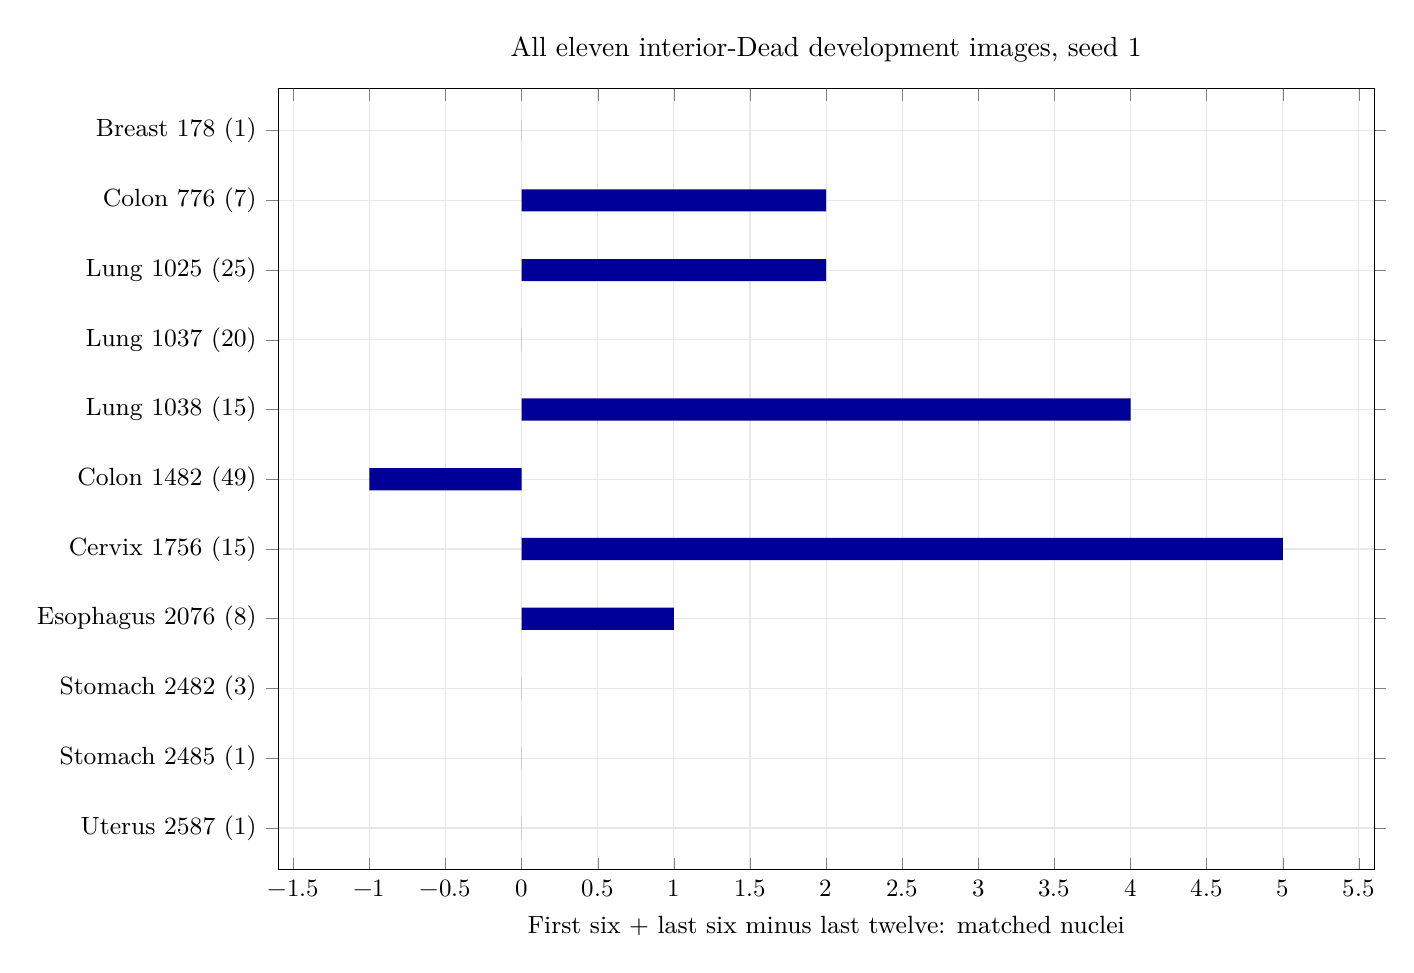
\begin{tikzpicture}
\begin{axis}[xbar,width=15.5cm,height=11.5cm,xlabel={First six + last six minus last twelve: matched nuclei},title={All eleven interior-Dead development images, seed 1},ytick={0,1,2,3,4,5,6,7,8,9,10},yticklabels={{Breast 178 (1)},{Colon 776 (7)},{Lung 1025 (25)},{Lung 1037 (20)},{Lung 1038 (15)},{Colon 1482 (49)},{Cervix 1756 (15)},{Esophagus 2076 (8)},{Stomach 2482 (3)},{Stomach 2485 (1)},{Uterus 2587 (1)}},ymin=-.6,ymax=10.6,y dir=reverse,bar width=8pt,grid=major,grid style={gray!18},tick label style={font=\small},label style={font=\small},title style={font=\normalsize}]
\addplot[fill=blue!60!black,draw=none] coordinates {(0,0) (2,1) (2,2) (0,3) (4,4) (-1,5) (5,6) (1,7) (0,8) (0,9) (0,10)};
\end{axis}
\end{tikzpicture}

\caption{Seed 1: all target-positive images}
\end{figure}

Seed 1 gains on five images, loses one and is unchanged on five. Lung
contributes +6, cervix +5, colon +1 and esophagus +1. Lung image 1038
contributes +4 in seed 1 and +5 in seed 19. Cervix 1756 contributes
+5/+2. Colon 1482 instead changes 11/49→10/49 in seed 1 and 13/49→13/49
in seed 19: 39/36 target objects remain missed in this concentrated
image. Lung 1025 reverses direction between seeds, −2/+2. Both seeds
improve in the aggregate, but their gains are distributed differently.
Removing any single positive image leaves gains of 6.15--14.58
percentage points in seed 1, alongside 8.03--16.67 in seed 19.

\begin{figure}[H]\centering
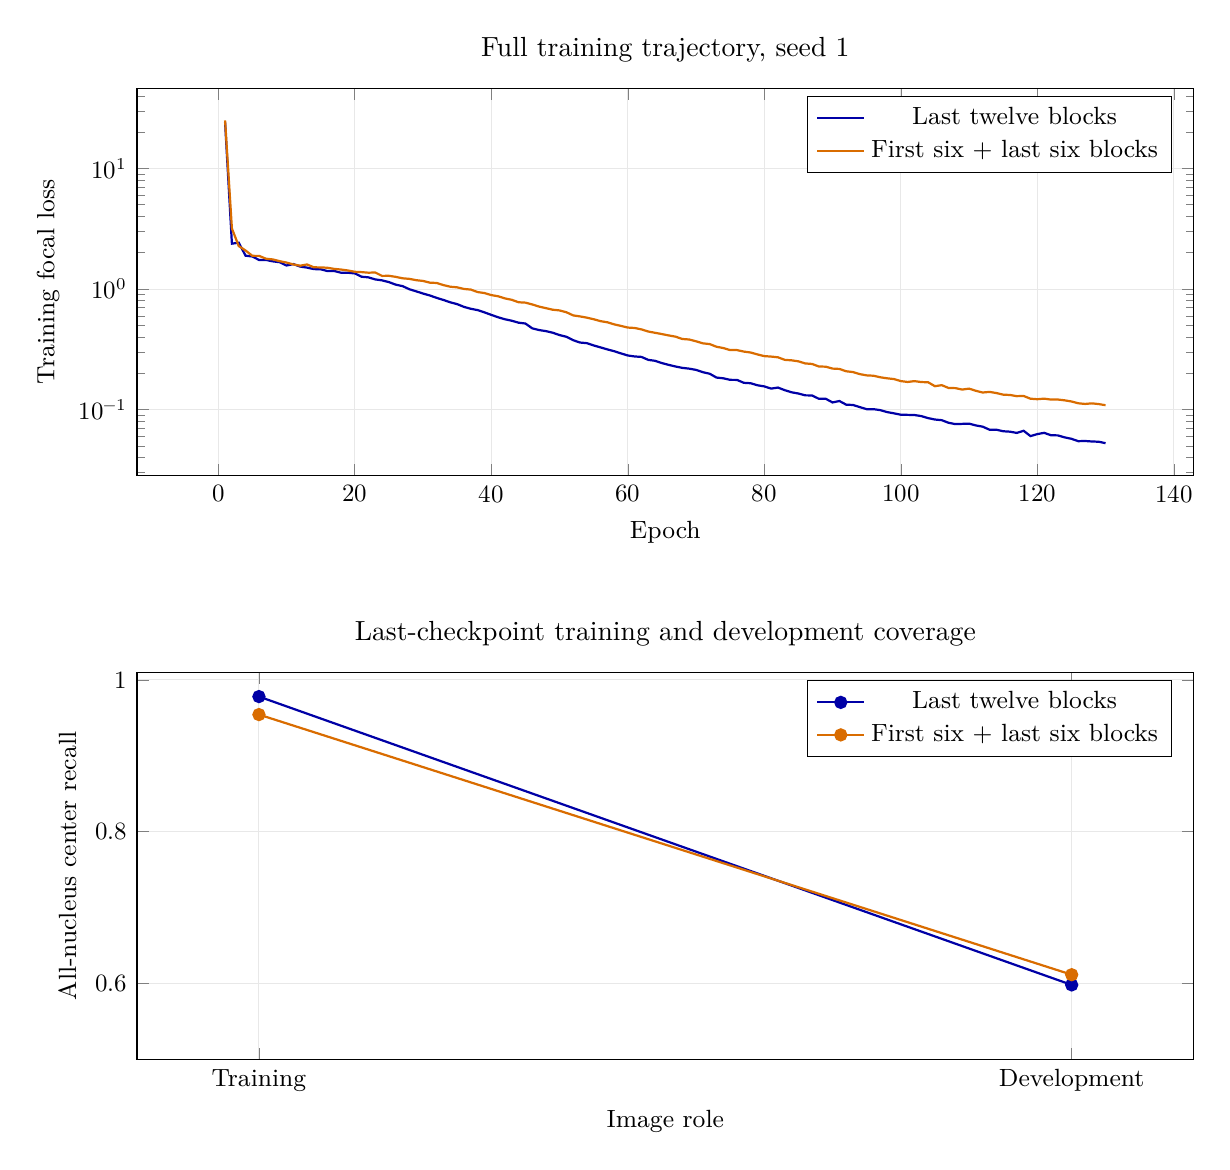
\begin{tikzpicture}
\begin{groupplot}[group style={group size=1 by 2,vertical sep=2.5cm},width=15cm,height=6.5cm,grid=major,grid style={gray!18},legend style={font=\small},tick label style={font=\small},label style={font=\small},title style={font=\normalsize}]
\nextgroupplot[xlabel={Epoch},ylabel={Training focal loss},ymode=log,title={Full training trajectory, seed 1}]
\addplot[thick,color=blue!65!black] coordinates {(1,24.1464097734) (2,2.37907460558) (3,2.42395087085) (4,1.89138898435) (5,1.86317232623) (6,1.74016351449) (7,1.74304416577) (8,1.69685451805) (9,1.67006233835) (10,1.56766110955) (11,1.61067377605) (12,1.53629610102) (13,1.50642142742) (14,1.46387814283) (15,1.45853354044) (16,1.41012065469) (17,1.41155984639) (18,1.36500526315) (19,1.36530261288) (20,1.34831311802) (21,1.26601811308) (22,1.25017444218) (23,1.20228692476) (24,1.18028517604) (25,1.1418605139) (26,1.08759826323) (27,1.05754919494) (28,0.996463930121) (29,0.957315703475) (30,0.917854604012) (31,0.884611722316) (32,0.844783207316) (33,0.811727376824) (34,0.776253122491) (35,0.749918353982) (36,0.711522315581) (37,0.686212550342) (38,0.669188185367) (39,0.640575755677) (40,0.610953438793) (41,0.583465234451) (42,0.561700555565) (43,0.546217831615) (44,0.526078422094) (45,0.517960491947) (46,0.472479875761) (47,0.457218615077) (48,0.447917287302) (49,0.434525593117) (50,0.415261976218) (51,0.402127236924) (52,0.376605498303) (53,0.36019223948) (54,0.35605725737) (55,0.340845657169) (56,0.328337270135) (57,0.315999150119) (58,0.305300156355) (59,0.292695673722) (60,0.281272957718) (61,0.276108612035) (62,0.273762871861) (63,0.258717186539) (64,0.25410910973) (65,0.243317074278) (66,0.235023784918) (67,0.227832109364) (68,0.222026201752) (69,0.218754308852) (70,0.213573085317) (71,0.204481938093) (72,0.198484528042) (73,0.184561390548) (74,0.181954261069) (75,0.176659237433) (76,0.176465889512) (77,0.166919391089) (78,0.165605806076) (79,0.159267719343) (80,0.155895322193) (81,0.149444878387) (82,0.152472293931) (83,0.145000228475) (84,0.13933104506) (85,0.136019747531) (86,0.131397780628) (87,0.131108616685) (88,0.122979612943) (89,0.123099924053) (90,0.114715974734) (91,0.117932853594) (92,0.109995811722) (93,0.10931592318) (94,0.104908588645) (95,0.100949496105) (96,0.100945127414) (97,0.0990364957451) (98,0.0954205769698) (99,0.0931880944945) (100,0.0907757309053) (101,0.0905180393667) (102,0.0902303193452) (103,0.088424334828) (104,0.0850573193147) (105,0.0828130932458) (106,0.0817788428467) (107,0.0778135305542) (108,0.0758810507128) (109,0.076215800676) (110,0.0765656325285) (111,0.073964573264) (112,0.0722589833385) (113,0.0681890490755) (114,0.0681911942967) (115,0.0661841659039) (116,0.0656570426451) (117,0.0641314384799) (118,0.0668080432189) (119,0.0603444048726) (120,0.0626898991414) (121,0.0642267048966) (122,0.0613357394715) (123,0.0611648887737) (124,0.0588851603053) (125,0.0573119477154) (126,0.0547676310772) (127,0.0549531287133) (128,0.0544491219801) (129,0.0541878870772) (130,0.052713020613)};
\addlegendentry{Last twelve blocks}
\addplot[thick,color=orange!85!black] coordinates {(1,25.011496911) (2,3.17799959623) (3,2.27436188492) (4,2.08865700683) (5,1.885834561) (6,1.8839197844) (7,1.78421891875) (8,1.76084290541) (9,1.70301685874) (10,1.65851540155) (11,1.59998793002) (12,1.56235476789) (13,1.59959509592) (14,1.51503495644) (15,1.51149311659) (16,1.50238437958) (17,1.4696641211) (18,1.45096074566) (19,1.42595314957) (20,1.39012699037) (21,1.38180783916) (22,1.36672399956) (23,1.37209300751) (24,1.28553308058) (25,1.28794003566) (26,1.26253414447) (27,1.22821307152) (28,1.21486726833) (29,1.18446103696) (30,1.16763180768) (31,1.12988207348) (32,1.12319189014) (33,1.07810610866) (34,1.04555361918) (35,1.033199504) (36,1.00191194403) (37,0.990080934014) (38,0.944060752715) (39,0.926574528371) (40,0.891300759756) (41,0.871630537951) (42,0.836584058926) (43,0.81430716645) (44,0.77721205911) (45,0.771726598473) (46,0.745692780707) (47,0.715607827831) (48,0.694585677345) (49,0.67398442983) (50,0.665043073873) (51,0.64224857131) (52,0.604723203274) (53,0.593133849232) (54,0.579252798606) (55,0.562060371949) (56,0.541903383772) (57,0.530444192252) (58,0.509721531137) (59,0.494748991699) (60,0.47940543766) (61,0.475636233514) (62,0.462900746059) (63,0.444441580239) (64,0.43372605681) (65,0.423428376604) (66,0.412513215189) (67,0.402878855115) (68,0.385366324147) (69,0.381752724151) (70,0.368892222992) (71,0.354728576386) (72,0.34968104504) (73,0.332328972624) (74,0.324155154326) (75,0.311755497574) (76,0.311781367654) (77,0.303075165604) (78,0.297676424355) (79,0.287003625485) (80,0.277921598474) (81,0.275451032265) (82,0.271752992647) (83,0.25877414053) (84,0.256390396781) (85,0.251566645488) (86,0.241655978028) (87,0.239265075389) (88,0.227968502746) (89,0.227136093183) (90,0.218998449615) (91,0.217567150648) (92,0.208101390862) (93,0.204921622139) (94,0.196992543635) (95,0.192389015248) (96,0.19113709086) (97,0.185506416595) (98,0.181884586101) (99,0.17933309276) (100,0.172520445635) (101,0.16965263944) (102,0.172393440965) (103,0.169369802517) (104,0.168656573035) (105,0.156491421992) (106,0.159630250606) (107,0.151222903264) (108,0.150808054505) (109,0.146756133286) (110,0.149384039095) (111,0.143327694706) (112,0.138696835582) (113,0.140289669869) (114,0.137317749343) (115,0.133153271166) (116,0.132303883946) (117,0.129376130577) (118,0.129833591042) (119,0.123228266547) (120,0.122043808987) (121,0.123365918834) (122,0.121185603338) (123,0.121300019186) (124,0.119477846619) (125,0.116899685834) (126,0.112925518259) (127,0.111518024011) (128,0.112746420551) (129,0.11120598165) (130,0.108816306706)};
\addlegendentry{First six + last six blocks}
\nextgroupplot[xlabel={Image role},ylabel={All-nucleus center recall},title={Last-checkpoint training and development coverage},xtick={0,1},xticklabels={Training,Development},xmin=-.15,xmax=1.15,ymin=.5,ymax=1.01]
\addplot[thick,mark=*,color=blue!65!black] coordinates {(0,0.978025427719) (1,0.598285714286)};
\addlegendentry{Last twelve blocks}
\addplot[thick,mark=*,color=orange!85!black] coordinates {(0,0.954324281902) (1,0.611755102041)};
\addlegendentry{First six + last six blocks}
\end{groupplot}
\end{tikzpicture}

\caption{Seed 1 training and development coverage}
\end{figure}

Training recall falls from 97.80\% to 95.43\%, and training Dead matches
from 624/656 to 606/656. Recorded training time is 4.0143 versus 6.7220
hours; checkpoint time is 238.77 versus 2,116.75 seconds. The seed-1
intervention was exposed to prolonged Lustre delays, and its application
completion time is 10.1409 hours. These elapsed timings include stalls
and provide a resource record, while the seed-19 21.24\% training
increase is the cleaner same-round cost comparison. GPU peaks are the
same across seeds: about 4.05 versus 4.84 GiB.

\subsection{Fixed objects that replicate, reverse or exchange across
seeds}\label{fixed-objects-that-replicate-reverse-or-exchange-across-seeds}

The fixed eight images in seed 1 retain 29 objects, gain 7, lose 3 and
miss 14 in both arms, for net +4 out of 53. Together with seed 19's
retained 30, gained 6, lost 4 and jointly missed 13, they expose local
changes behind the aggregate improvement.

\noindent

\begin{minipage}{\linewidth}\centering
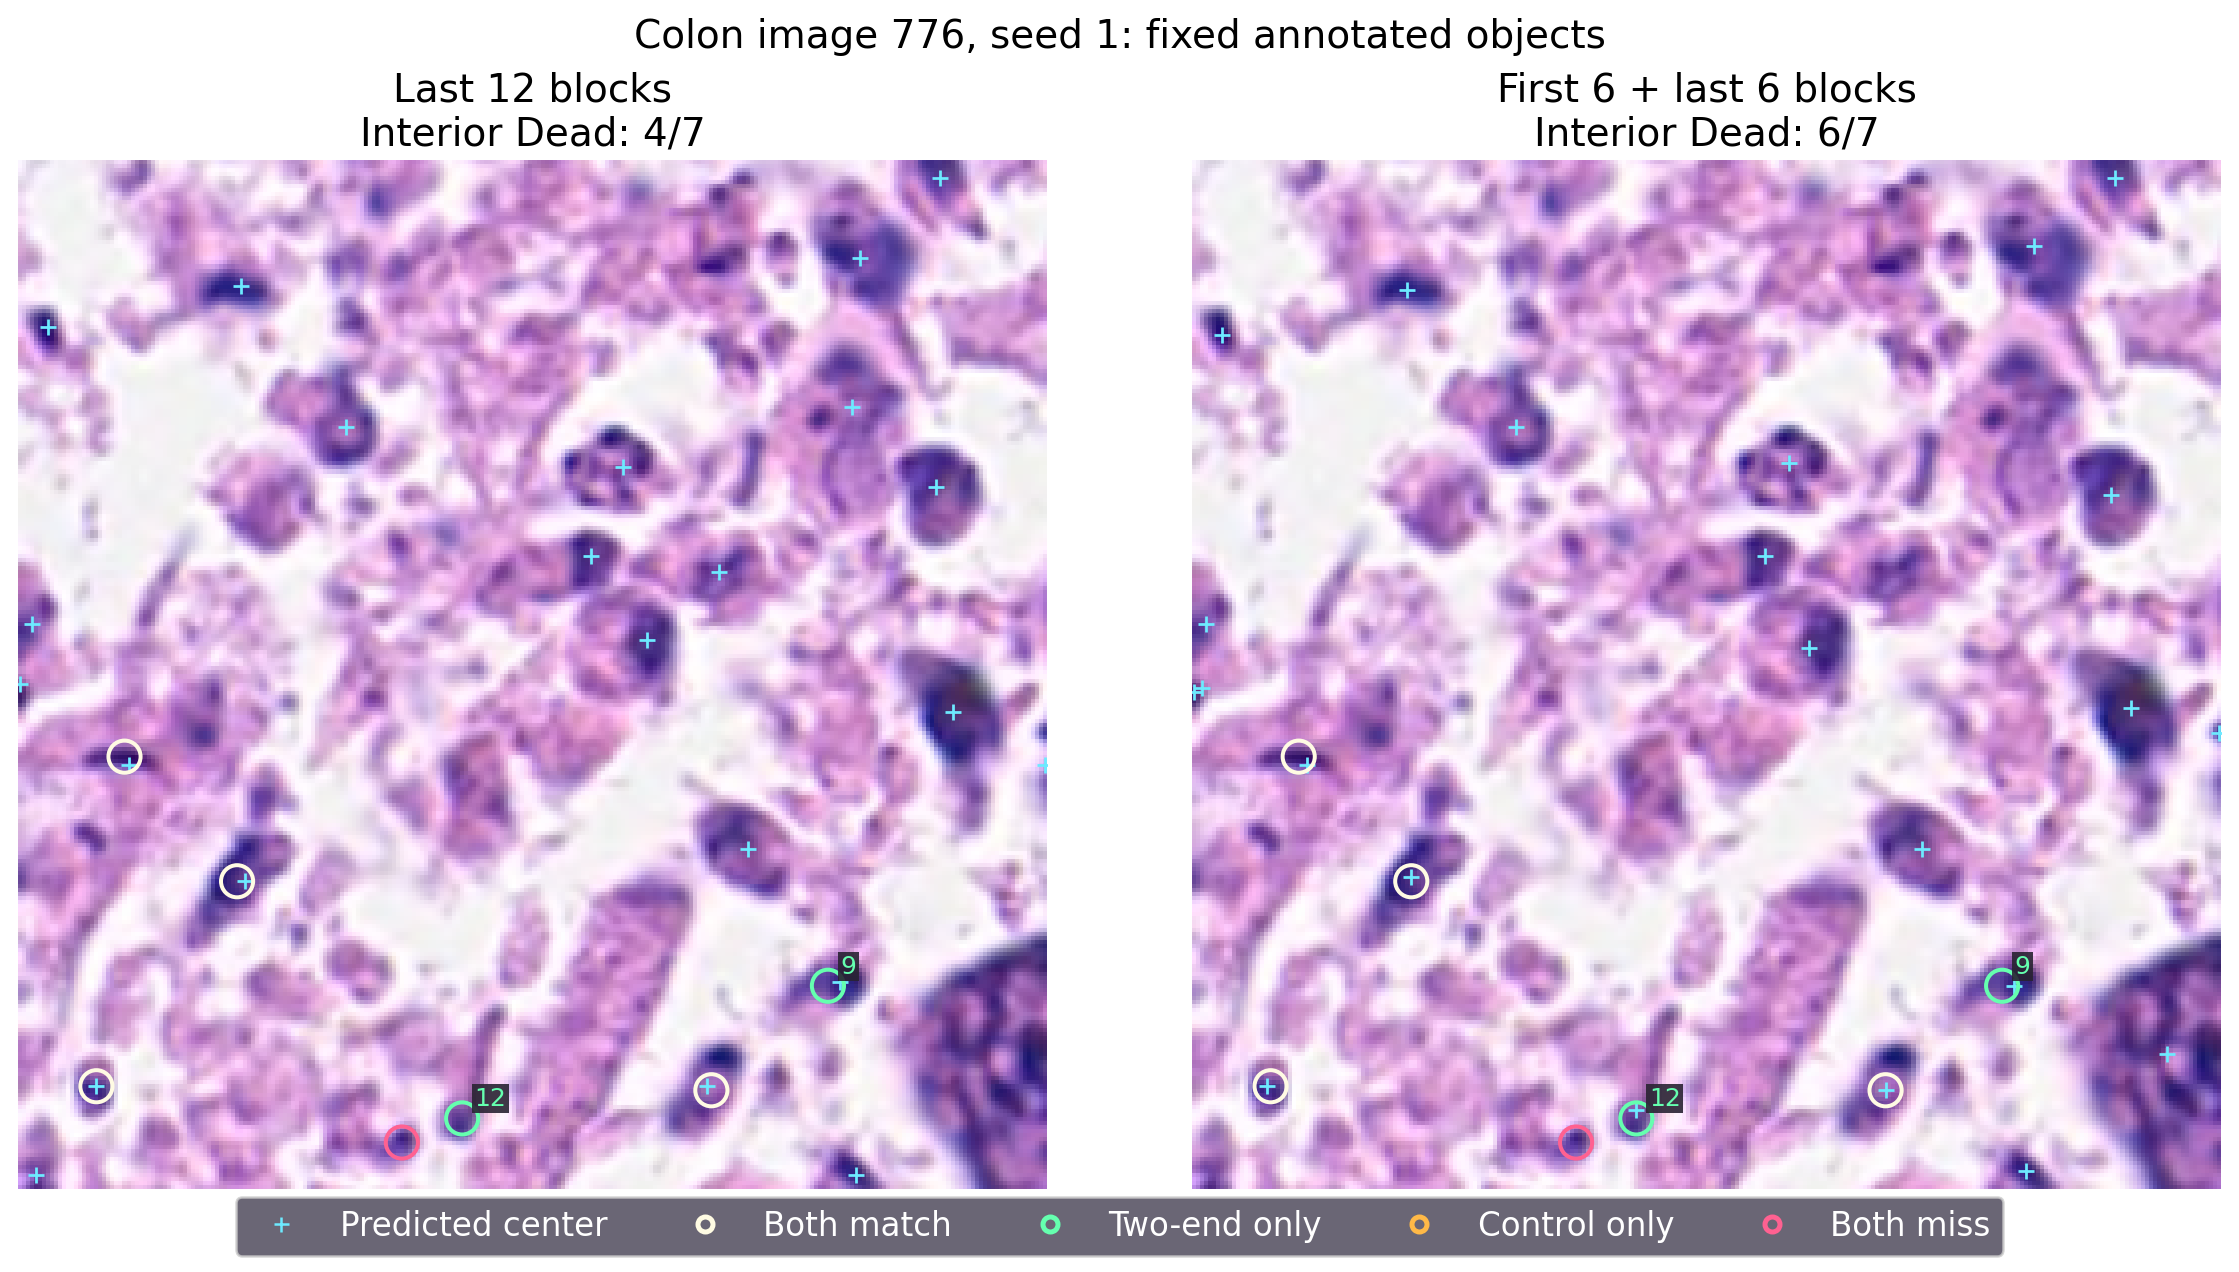
\includegraphics[width=\linewidth,height=0.40\textheight,keepaspectratio]{../figures/p29_image_776_seed_1.png}
\captionof{figure}{Seed 1, colon 776}
\raggedright

Colon 776 improves 4/7→6/7. Object 12 at (238,110), area 104, is recovered in both seeds: its nearest prediction moves 61.52→2.00 pixels in seed 1 and 80.66→1.00 in seed 19. This shared recovery provides a concrete repeatable example at the same annotation. Seed 1 also gains object 9 at (205,201), area 191, as its distance crosses 3.16→3.00 pixels. Seed 19 instead gains objects 10 and 11 in the lower strip, demonstrating that the same total benefit can involve different nuclei.

\end{minipage}

\noindent

\begin{minipage}{\linewidth}\centering
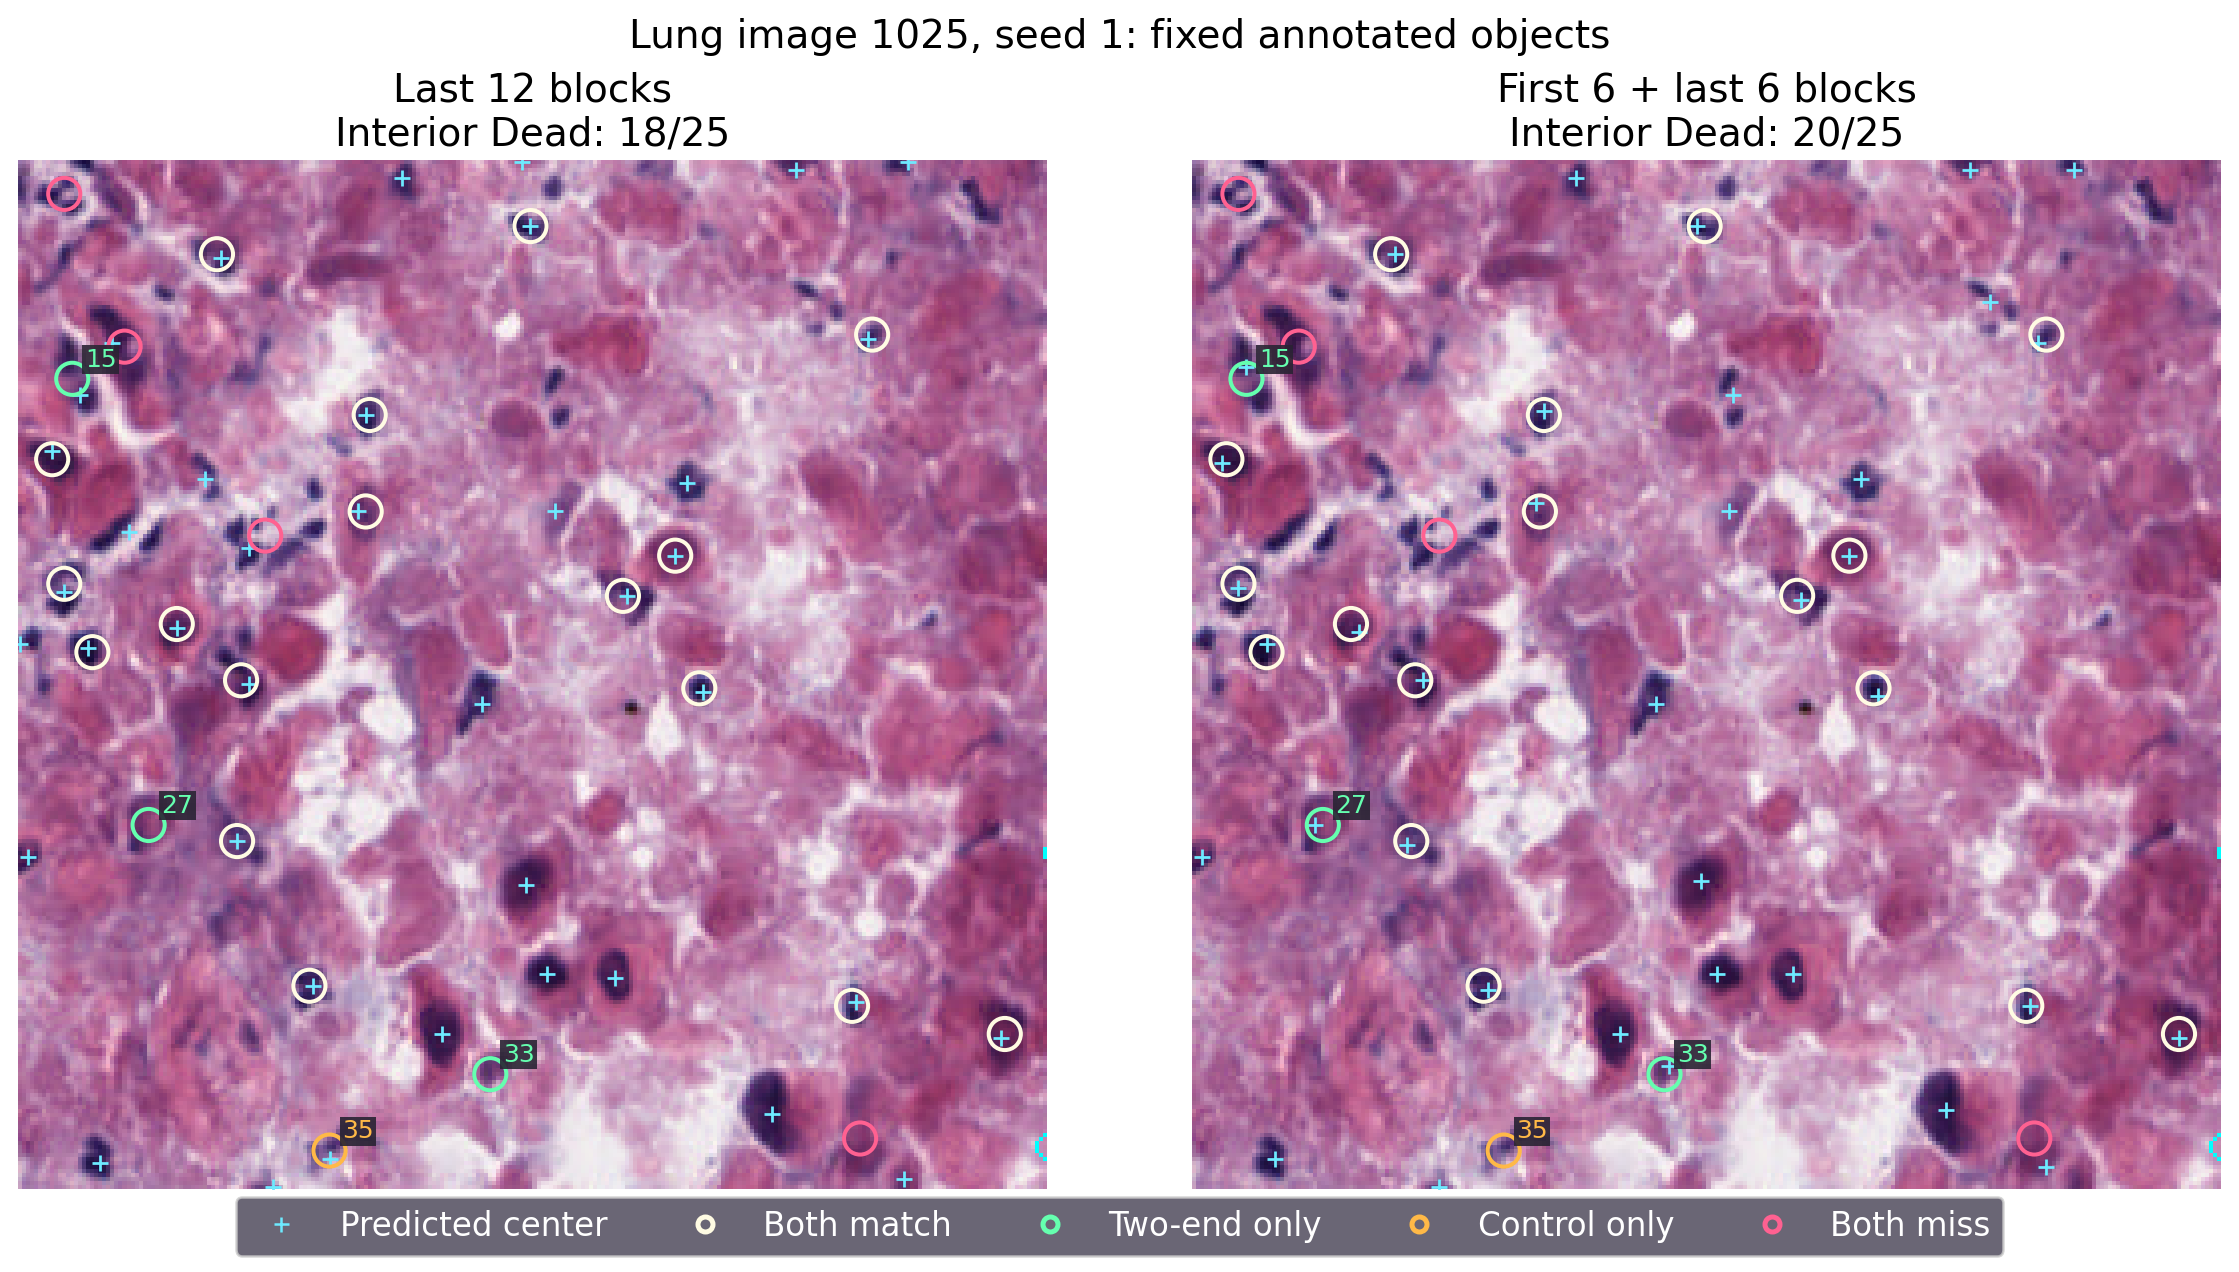
\includegraphics[width=\linewidth,height=0.40\textheight,keepaspectratio]{../figures/p29_image_1025_seed_1.png}
\captionof{figure}{Seed 1, lung 1025}
\raggedright

Lung 1025 improves 18/25→20/25 in seed 1. Objects 15 (54,13), 27 (165,32) and 33 (227,117) are gained, with distances 4.47→3.00, 22.36→2.00 and 15.62→2.24 pixels. Object 33 has area 52, placing it in the predefined small-object subset. Object 35 (246,77), area 68, is lost in both seeds: 2.00→18.36 in seed 1 and 1.00→18.36 in seed 19. That repeated loss coexists with the positive tissue-level aggregate.

\end{minipage}

\noindent

\begin{minipage}{\linewidth}\centering
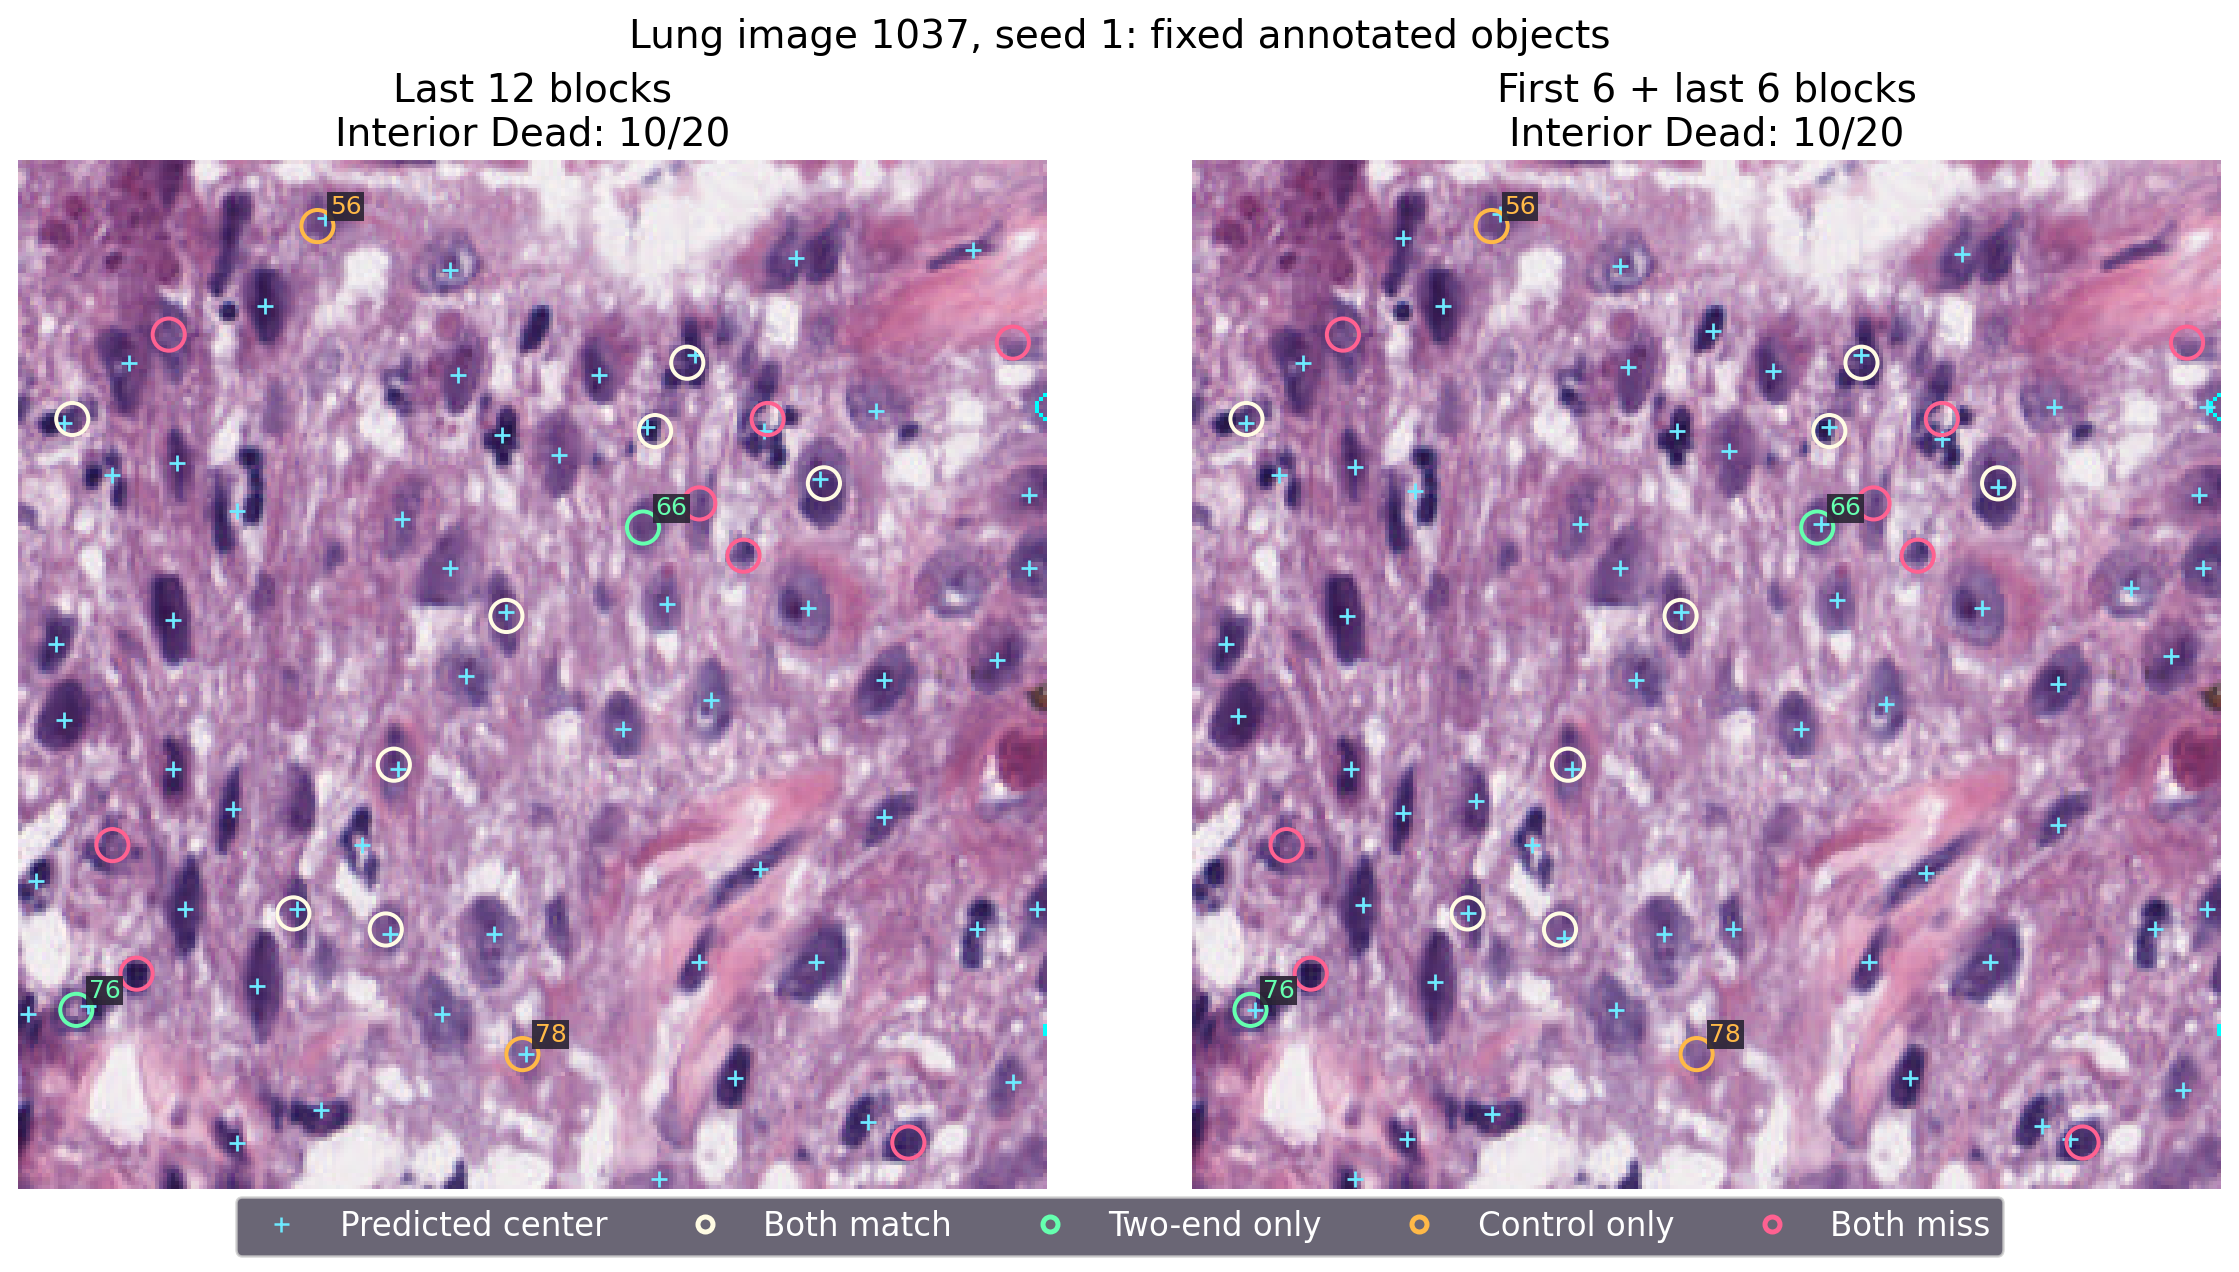
\includegraphics[width=\linewidth,height=0.40\textheight,keepaspectratio]{../figures/p29_image_1037_seed_1.png}
\captionof{figure}{Seed 1, lung 1037}
\raggedright

Lung 1037 stays at 10/20 in seed 1, exchanging two gains and two losses. Objects 66 (91,155) and 76 (211,14) gain predictions at distances 19.92→1.41 and 3.16→1.00; objects 56 (16,74) and 78 (222,125) lose matches at 2.83→3.61 and 1.00→22.83. Object 56 crosses the identical boundary in both seeds. An unchanged image count can therefore conceal repeated localization loss plus compensating recovery elsewhere. All object distances, original centers and one-to-one assignments are included in the CSV and raw coordinate JSONs.

\end{minipage}

\subsection{Research and preservation
decisions}\label{research-and-preservation-decisions}

The next fixed experiment isolates the middle twelve blocks, filling the
remaining contiguous update-position comparison. It retains the
151,179,264 trainable encoder parameters, 3,294,657 head parameters,
original rates, 130 epochs, seeds, cohort and decision rule. Its
hardware checks must demonstrate that data gradients reach middle blocks
through the frozen suffix and that the frozen blocks remain unchanged.
This is an adaptive development experiment with results to be reported
regardless of outcome.

The combined scientific collection verifies 92 small payloads, including
48 final PNGs, against their collected SHA256 values. The 505
source-file verification is inherited from the verified seed-19
collection. Seed-19 and control seed-1 payloads match original
preservation records. Experimental seed 1 timed out during preservation
after model completion. CPU recovery job 55745860 completed in 185
seconds and preserved all 23 run files, including both checkpoints and
12 final PNGs, with source hashes and independent target readback. All
21 small files match the earlier collection. Six other checkpoint sizes
match original records; independent rehashing of those six and external
archival remain outstanding.
\href{../P29_PRESERVATION_RECOVERY.json}{Preservation recovery} records
the verified checkpoint hashes.
\href{../p29_verified_analysis.json}{Machine-readable analysis},
\href{../object_summary.json}{object changes},
\href{../stage_pairs.csv}{stage pair table}, and
\href{../collection_result.json}{collection verification} accompany the
report. Both seed-level original decisions are false. Close this fixed
first-six plus last-six recipe under the original rule. Its paired gains
motivate the separately frozen middle-twelve development comparison.

\end{document}
